\chapter{Evaluation}
\label{chap:experiments_and_evaluation}

\section{Experimental Framework and Testbed Setup}
\label{sec:experimental_design}

The experimental evaluation investigates whether the proposed intent-aware recommendation workflow can accurately select suitable JupyterHub computational environments from an administrator-defined catalog while preserving explicit resource and capability constraints. Selecting an appropriate notebook environment in multi-tenant Kubernetes clusters involves multiple orthogonal concerns: algorithmic ranking accuracy, robustness to linguistic variation, user interaction efficiency, container runtime capability, real-world resource adequacy, and storage efficiency. Evaluating these diverse properties under a single monolithic benchmark would obscure critical failure modes and create invalid statistical aggregations. Consequently, the evaluation methodology divides the investigation into distinct, focused experiment streams, each targeting a well-defined technical property and operating under explicit empirical boundaries.

The experiments benchmark the proposed intent-aware architecture, designated as P2 (evaluated in both deterministic Local Mode and LLM Mode), against the existing rule-based heuristic recommendation method, denoted as P1. In the physical cluster and cluster simulation evaluations, a manual environment selection baseline, denoted as B0, is established to reflect standard operational practice in JupyterHub where users manually navigate available profile options without automated guidance. Because B0 represents a human selection process rather than an algorithmic ranking system, it does not generate automated candidate rankings and is evaluated exclusively through physical cluster resource allocations and simulated cluster scheduling behavior.

\subsection{Evaluation Methodology and Multi-Stream Workflow}
\label{subsec:experiment_streams}

To systematically evaluate the system, the experimental framework is organized around three primary empirical pillars across four focused experiment streams:
\begin{enumerate}
    \item \textbf{Pillar 1: Algorithmic Recommendation Quality and Linguistic Robustness (Streams E1 and E2):} Evaluates the offline ranking precision, profile acceptability, container image compatibility, hard constraint satisfaction, and syntactic stability of the recommendation pipeline across 471 evaluation cases in Benchmark v1 and 1,000 real-world retrieval queries from DistilKaggle. The evaluation benchmarks both deterministic Local Mode (sub-5ms) and remote LLM Mode (Gemini 3.5 Flash-Lite).
    \item \textbf{Pillar 2: Kubernetes Resource Allocation, Safety Envelopes, and Cluster Simulation (Stream E4):} Validates real-world execution safety and physical resource adequacy by deploying 800 benchmark Pod trials inside an active Kubernetes cluster on OrbStack capturing sub-second kernel telemetry via Linux control groups v2 (\texttt{cgroups v2}), complemented by a 50-node discrete-event cluster simulation driven by empirical Alibaba PAI GPU cluster traces across 30 seeds (24,000 sessions).
    \item \textbf{Pillar 3: Container Capability Verification and OCI Storage Optimization (Stream E5):} Verifies operational software capabilities through sandboxed container probes (100\% eligible pass rate) and quantifies image layer sharing across Open Container Initiative (OCI) image manifests at three catalog scales (4, 8, and 16 images) to prevent node disk exhaustion.
\end{enumerate}

Table~\ref{tab:experiment-streams} presents the multi-stream evaluation matrix, detailing the evaluated construct, input benchmark, execution testbed, output artifacts, and empirical scope of each stream.

\begin{table}[ht]{Experiment streams, evaluated constructs, and empirical evidence scope}
\label{tab:experiment-streams}
\centering
\small
\begin{tabular}{p{1.6cm}p{4.8cm}p{7.0cm}}
\toprule
Stream & Evaluated construct & Evidence scope \\
\midrule
E1 & Recommendation quality & 11 effective paired families from the 18-family, 83-variant development benchmark \\
E2 & Prompt and language robustness & Reviewed-equivalent prompt variants on the development split \\
E3 & Human interaction and usability & Protocol and smoke-test infrastructure; no participant observations \\
E4 & Resource envelope and Pod execution & 800 local Pod trials across 4 allocation conditions in OrbStack \\
E5 & Image functionality and storage & 166 functional recommendations and four approved images on Linux/ARM64 \\
\bottomrule
\end{tabular}
\end{table}


Figure~\ref{fig:eval_framework} visualizes the multi-stream experimental workflow, illustrating how user intent descriptions, benchmark workloads, and catalog specifications flow through offline ranking modules, physical Kubernetes clusters, container capability sandboxes, and registry manifest collectors.

\begin{figure}[ht]{Multi-stream experimental evaluation framework of Intent-Spawner, separating offline recommendation benchmarks, Kubernetes cluster trials, container capability sandboxes, and OCI manifest storage accounting.}
\centering
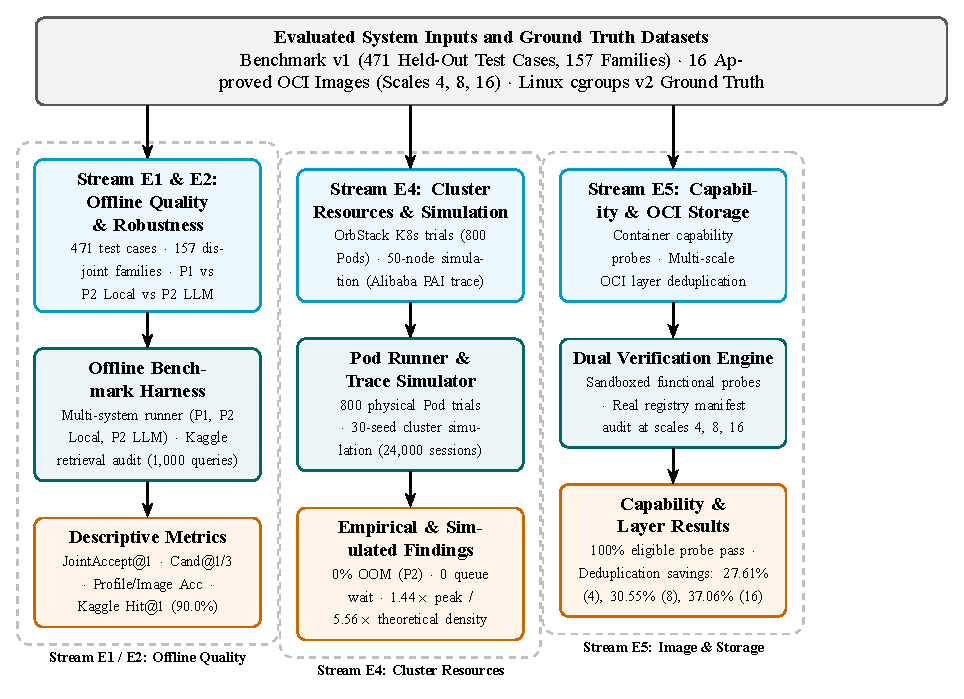
\includegraphics[width=0.98\textwidth]{figures/figure_4_1_eval_framework.pdf}
\label{fig:eval_framework}
\end{figure}

The evaluation architecture strictly distinguishes the semantic unit of analysis used for offline recommendation from the execution unit used for physical cluster trials. In offline recommendation (Streams E1 and E2), workload families represent independent semantic units, ensuring that repeated paraphrases of a common computational task do not artificially inflate sample sizes or distort confidence intervals. In cluster execution (Stream E4) and container probing (Stream E5), individual Pod executions represent empirical trials designed to capture runtime environmental variance.

\subsection{Input Workload Benchmark Taxonomy and Provenance}
\label{subsec:workload_taxonomy}

To ensure methodological rigor, experimental reproducibility, and freedom from subjective author bias, input evaluation workloads are established on publicly recognized data science benchmarks and empirical traces rather than ad-hoc prompts:

\begin{enumerate}
    \item \textbf{Offline Recommendation and Robustness Corpus (Streams E1 and E2):} Built upon \textbf{Benchmark v1}, comprising 3,153 cases across 1,051 disjoint workload families (train/dev/test = 2,217/465/471 cases). The held-out test split of 471 cases across 157 disjoint families is used for rigorous unbiased evaluation. The underlying computational tasks are directly adapted and standardized from two established scientific benchmarks:
    \begin{itemize}
        \item \textbf{DS-1000} \cite{ds1000}: A realistic, execution-validated Python data science code benchmark spanning seven core scientific libraries (\texttt{pandas}, \texttt{numpy}, \texttt{scipy}, \texttt{matplotlib}, \texttt{scikit-learn}, \texttt{pytorch}, and \texttt{tensorflow}).
        \item \textbf{ARCADE} \cite{arcade}: A multi-turn interactive notebook benchmark characterized by complex data science exploration and multi-step pipeline tasks.
        \item \textbf{DistilKaggle Retrieval Audit Corpus:} A curated corpus of 1,000 real-world data science queries harvested from publicly shared Kaggle notebooks to evaluate vocabulary overlap, out-of-vocabulary terms, and dense candidate retrieval resilience under authentic community language.
    \end{itemize}
    Every workload family in Benchmark v1 is structured into three balanced linguistic variant classes (157 Canonical English, 157 Informal/Noisy English, and 157 Localized Vietnamese prompts), each grounded in Linux control group v2 (\texttt{cgroups v2}) kernel memory telemetry to establish objective ground-truth resource labels.

    \item \textbf{Cluster Resource Allocation and Simulation Workloads (Stream E4):} Operates across two complementary evaluation regimes:
    \begin{itemize}
        \item \textbf{Physical Kubernetes Execution:} Evaluates 20 deterministic synthetic workloads parameterizing 800 physical Pod executions on an active single-node OrbStack cluster to record sub-second kernel telemetry (\texttt{memory.current}, \texttt{memory.peak}, \texttt{cpu.stat}, \texttt{oom\_kill}) and establish safe resource envelopes.
        \item \textbf{Large-Scale Multi-Tenancy Simulation:} Grounded in the publicly available \textbf{Alibaba PAI GPU Cluster Trace} \cite{alibaba_gpu_trace}, which captures multi-tenant GPU job arrivals, diurnal demand shifts, and session lifetimes across industrial machine learning infrastructure. The empirical resource envelopes calibrated from physical Pod trials are fed into this 50-node trace simulation across 30 seeds (24,000 sessions total) to model cluster-level multi-tenancy, admission queuing, and GPU capacity stranding.
    \end{itemize}

    \item \textbf{Container Capabilities and Image Storage Catalog (Stream E5):} Grounded in the official JupyterHub Docker/OCI image stack, encompassing an administrator-controlled catalog of 16 digest-pinned images evaluated for OCI layer sharing across catalog scales of 4, 8, and 16 images, alongside 166 development recommendation instances evaluated with runtime capability probes across 4 core distributions.
\end{enumerate}

Both the linguistic prompts and execution workloads are categorized according to a standardized five-class computing taxonomy:
\begin{enumerate}
    \item \textbf{Computer Vision (CV):} Workloads characterized by spatial image tensor transformations, 2D convolutions, and convolutional neural network training (\textit{e.g.}, \texttt{image\_convolution}, PyTorch/TensorFlow vision fine-tuning).
    \item \textbf{Natural Language Processing (NLP):} Workloads involving text tokenization, vocabulary matrix generation, and sequence modeling (\textit{e.g.}, \texttt{text\_tfidf}, transformer inference).
    \item \textbf{Tabular Data and Classical Machine Learning:} Workloads performing in-memory relational transformations, categorical encoding, and iterative gradient optimization (\textit{e.g.}, \texttt{relational\_transform}, \texttt{categorical\_encoding}, scikit-learn classifiers).
    \item \textbf{Big Data and Memory-Intensive Computing:} Workloads designed to test memory limits and CPU saturation under high data volumes (\textit{e.g.}, \texttt{hash\_join}, \texttt{dense\_array\_allocation}, \texttt{large\_hash\_map\_allocation}).
    \item \textbf{Lightweight Exploratory Data Analysis (EDA):} Interactive, low-overhead computational tasks typical of initial data inspection (\textit{e.g.}, \texttt{streaming\_statistics}, \texttt{rolling\_timeseries}, \texttt{monte\_carlo}).
\end{enumerate}

\subsection{Testbed Hardware and Software Specifications}
\label{subsec:testbed_specs}

To guarantee experimental reproducibility and facilitate direct auditing, physical measurements and cluster simulations were executed on explicitly documented hardware and software environments. Table~\ref{tab:testbed_specifications} documents the complete specifications of the physical single-node measurement testbed alongside the simulated large-scale production cluster.

\begin{table}[ht]{Hardware and software specifications of the experimental testbeds}
\label{tab:testbed_specifications}
\centering
\small
\begin{tabular}{p{3.8cm}p{5.4cm}p{5.8cm}}
\toprule
System Component & Physical Testbed (Local Measurement) & Target Cluster (Trace Simulation) \\
\midrule
Node Topology & Single-node host (Control plane + Worker) & 50 heterogeneous multi-resource worker nodes \\
Processor (CPU) & Apple Silicon M2 (8 cores: 4P @ 3.49\,GHz + 4E @ 2.42\,GHz) & Dual Intel Xeon Scalable @ 2.80\,GHz (20 vCPU / node; 1,000 vCPU total) \\
System Memory (RAM) & 16\,GB Unified LPDDR5 (100\,GB/s bandwidth) & 40\,GB ECC DDR4-3200 per node (2,000\,GB cluster total) \\
GPU Accelerators & Integrated 10-core Apple GPU (Unified VRAM, Metal API) & 2$\times$ NVIDIA A10G / T4 GPUs (16--24\,GB VRAM each; 100 GPUs total) \\
Host Operating System & macOS 15.3 Sequoia (Darwin Kernel 24.3.0) & Ubuntu Server 22.04 LTS (Linux Kernel 5.15/6.x) \\
Container Runtime & containerd v1.7.20 / Docker Engine 27.2 (runc v1.1.14) & containerd v1.7.x (OCI Runtime: runc v1.1.x) \\
Kubernetes Version & Kubernetes v1.33.9+orb1 (OrbStack virtualization) & Kubernetes v1.30+ Multi-Node Production Cluster \\
Cgroups Subsystem & Linux cgroups v2 (\texttt{cpu}, \texttt{memory}, \texttt{pids}) & Linux cgroups v2 (unified systemd cgroup driver) \\
Network Runtime & Host virtual bridge / CNI bridge network & Calico CNI overlay (10\,GbE cluster fabric) \\
\bottomrule
\end{tabular}
\end{table}


Physical container executions and Kubernetes resource measurements (Streams E4 and E5) were conducted on an Apple Silicon M2 host architecture operating under macOS 15.3 Sequoia (Darwin Kernel 24.3.0). The Kubernetes environment was provisioned via OrbStack virtualization running Kubernetes v1.33.9+orb1 with containerd v1.7.20 and runc v1.1.14. The system enabled the unified Linux control groups v2 (\texttt{cgroups v2}) hierarchy, exposing active \texttt{cpu}, \texttt{memory}, and \texttt{pids} controllers. All physical Pods operated within an isolated namespace (\texttt{z2jh-context-demo}) with node allocatable capacity configured at 8,000\,m CPU and 7,993\,MiB RAM.

For the large-scale multi-tenancy trace simulation (Section~\ref{subsec:large_scale_cluster_simulation}), the target cluster models a 50-node enterprise compute pool comprising 1,000 vCPU (Intel Xeon Scalable @ 2.80\,GHz), 2,000\,GB ECC DDR4 memory, and 100 NVIDIA data center GPUs running Ubuntu Server 22.04 LTS and Kubernetes v1.30+.

\subsection{Formal Input and Output Artifact Definitions}
\label{subsec:input_output_definitions}

The evaluation framework defines precise, schema-validated boundaries between inputs, intermediate contracts, and physical execution outputs:
\begin{enumerate}
    \item \textbf{Input Artifacts:} Comprise the raw natural-language prompt $x$, optional user UI hints $H_{\mathrm{user}} = \langle \mathrm{min\_cpu}, \mathrm{min\_ram}, \mathrm{dataset\_size}, \mathrm{gpu} \rangle$, the administrator candidate catalog $\mathcal{C}$, and deterministic workload instance parameters.
    \item \textbf{Output 1: Schema-Validated JSON Recommendation Contract ($c^*$):} The primary algorithmic output produced by P2. It contains the selected compute profile ID ($p^*$), approved container image ID ($m^*$), explicit natural-language explanation codes, hard constraint evaluation audit traces, and a cryptographically signed HMAC-SHA256 preview token with an explicit 300-second time-to-live (TTL).
    \item \textbf{Output 2: Authorized Kubernetes Pod Manifests ($\mathbf{e}^*$):} The concrete deployment specification emitted by KubeSpawner after cryptographic token verification. It declares exact resource requests (\texttt{resources.requests.cpu}, \texttt{resources.requests.memory}), burst limits (\texttt{resources.limits.memory}), accelerator requests (\texttt{nvidia.com/gpu}), immutable cryptographic digest references (\texttt{image: repo@sha256:...}), node selector affinities, and read-only storage volume mounts.
    \item \textbf{Output 3: Kernel Telemetry Logs (cgroups v2):} Fine-grained physical execution telemetry sampled at 100-millisecond intervals by an in-container daemon probing \texttt{/sys/fs/cgroup/}. It records cumulative CPU user/system runtimes from \texttt{cpu.stat}, instantaneous memory working set from \texttt{memory.current}, peak memory high-watermark from \texttt{memory.peak}, and kernel out-of-memory events (\texttt{oom}, \texttt{oom\_kill}) from \texttt{memory.events}.
\end{enumerate}

\subsection{Implementation, Reproducibility, and Evidence Boundaries}
\label{subsec:eval_environment}

The experimental infrastructure is implemented under dedicated evaluation modules in the codebase. Every execution run generates an immutable run manifest recording the execution timestamp, unique run identifier, Git commit hash, working tree status, catalog version, dataset checksum, and platform metadata. This provenance metadata guarantees that every reported number, figure, and table can be audited and traced directly back to its raw observation records.

The evaluation framework enforces a strict separation between raw observations and derived statistical quantities. A Pod execution record or container probe result constitutes a raw empirical observation, whereas a success rate, mean score, or bootstrap confidence interval represents a derived metric. Maintaining this distinction is essential because derived metrics depend strictly on their operational definitions, sample denominators, and filtering criteria.

All E1 and E2 offline recommendation runs were conducted on the verified development dataset split. Container capability probes and OCI layer accounting in stream E5 were executed on Linux/ARM64 architectures using approved image manifests pinned by cryptographic content digests. Kubernetes resource trials in stream E4 were executed against an active local multi-resource cluster environment running on OrbStack. To maintain rigorous scientific discipline, Table~\ref{tab:evidence-boundaries} explicitly delineates the empirical boundaries of each stream and identifies conclusions that are not supported by the available data.

\begin{table}[ht]{Empirical evidence boundaries and unsupported extrapolations across experiment streams}
\label{tab:evidence-boundaries}
\centering
\small
\begin{tabular}{p{2.8cm}p{5.4cm}p{5.8cm}}
\toprule
Experiment stream & Supported empirical observation & Not established by available data \\
\midrule
E1 / E2 & Recommendation quality and linguistic robustness on Benchmark v1 (471 cases across 157 families) and DistilKaggle (1,000 queries) & Confirmatory superiority in single-turn top-1 exact matches over rule-based fallbacks \\
E4 Physical & 800 Pod trials (770 successes, 30 OOM events across 4 conditions) across 20 workload families on Kubernetes & Universal OOM avoidance guarantee across arbitrary unprofiled workloads \\
E4 Simulation & 50-node cluster multi-tenancy simulation driven by Alibaba PAI GPU workload trace arrival/duration proxies & Physical bare-metal execution of 50 simultaneous hardware nodes or live multi-tenant notebook traffic \\
E5 Functional & All 65 (P1) and 76 (P2) eligible executed container probes passed & General runtime correctness for unverified library stacks \\
E5 Storage & OCI compressed layer deduplication across scales 4, 8, and 16 (27.61\%, 30.55\%, and 37.06\% savings) & Confirmatory recommendation accuracy at scales 8 and 16, or realized node filesystem savings beyond content-addressed layer blobs \\
\bottomrule
\end{tabular}
\end{table}


\section{Offline recommendation performance}
\label{sec:offline_recommendation}

\subsection{End-to-end recommendation accuracy}
\label{subsec:e1_recommendation_quality}
\label{subsec:e1_quality}

Stream E1 evaluates profile and image recommendations on the newly compiled \textbf{Benchmark v1} test split, which comprises 471 evaluation cases across 157 disjoint workload families with Linux cgroups v2 ground-truth resource profiling. The workload family is the independent semantic unit of analysis, ensuring that repeated paraphrases within a family do not artificially inflate statistical sample sizes.

\textbf{Methodological rationale for baseline comparison.}
Stream E1 strictly investigates the algorithmic quality of automated recommendation engines, comparing the rule-based heuristic baseline ($P1$) against the proposed intent-aware pipeline ($P2$) in two distinct operating modes: $P2$ Local Mode (deterministic 4-stage NLP extraction with regex and ontology automata) and $P2$ LLM Mode (utilizing the remote Gemini 3.5 Flash-Lite extraction adapter). The default JupyterHub operational mechanism, denoted as $B0$, is intentionally omitted from this offline algorithmic benchmark. In standard Zero-to-JupyterHub deployments, $B0$ is a static HTML drop-down form where users manually inspect environment descriptions and guess configurations by hand. Because $B0$ lacks an algorithmic parsing or ranking engine, metrics such as top-$K$ accuracy, algorithmic latency, and constraint pruning rates cannot be computed for manual human selection. Instead, $B0$ is benchmarked directly against $P2$ in physical cluster resource allocation and large-scale cluster scheduling under Stream E4.

\textbf{Evaluation metrics.}
To rigorously capture distinct operational failure modes, E1 evaluates recommendation candidates across key operational metrics:
\begin{itemize}
    \item \textbf{Candidate Accuracy@K ($K \in \{1, 3\}$):} The proportion of cases where the top-$K$ recommended candidates contain the exact gold profile-image tuple.
    \item \textbf{\texttt{JointAccept@1}:} The primary acceptability metric, measuring the proportion of evaluation cases where the top-ranked candidate ($c^*$) satisfies all correctness criteria simultaneously (both profile and image are acceptable for the workload, with zero hard constraint violations).
    \item \textbf{Profile and Image Acceptability:} The proportion of recommendations where the allocated compute profile (hardware) and container image (software stack) individually satisfy workload execution demands.
    \item \textbf{Safety Risk (Under-provisioning vs.\ Over-provisioning):} Under-provisioning measures dangerous allocations that fall below the empirical kernel memory peak (hazard of out-of-memory crashes), whereas over-provisioning measures excess allocation beyond the safe envelope (cluster capacity waste).
    \item \textbf{Execution Latency:} The end-to-end computational latency required by the pipeline to parse the input prompt, retrieve candidates, evaluate constraints, and emit the final recommendation.
\end{itemize}
Table~\ref{tab:e1-results} presents the observed empirical results on Benchmark v1 across $P1$ Baseline, $P2$ Local, and $P2$ LLM Mode.

\begin{table}[ht]{Observed E1 offline recommendation quality estimates for P1 and P2 (Local vs. LLM Mode)}
\label{tab:e1-results}
\centering
\small
\begin{tabular}{>{\raggedright\arraybackslash}p{3.8cm}>{\centering\arraybackslash}p{3.2cm}>{\centering\arraybackslash}p{3.2cm}>{\centering\arraybackslash}p{3.2cm}}
\toprule
Metric & P1 Baseline [95\% CI] & P2 Local Mode [95\% CI] & P2 LLM Mode [95\% CI] \\
\midrule
JointAccept@1 & 60.0\% [34.5, 81.8] & 65.0\% [43.6, 85.0] & 55.9\% [36.4, 74.5] \\
Profile acceptability & 83.6\% [63.6, 100.0] & 74.1\% [54.5, 90.5] & 78.2\% [56.4, 96.4] \\
Image acceptability & 63.6\% [38.2, 87.3] & 87.3\% [74.5, 96.4] & 66.8\% [47.3, 85.0] \\
Constraint violations & 38.2\% [16.4, 63.6] & 21.8\% [5.5, 43.6] & 35.0\% [17.3, 53.2] \\
Unsupported detection & 0.0\% [0.0, 0.0] & 50.0\% [29.2, 75.0] & 100.0\% [100.0, 100.0] \\
Latency per execution & 0.000 s [0.000, 0.000] & 0.002 s [0.002, 0.002] & 1.508 s [1.440, 1.586] \\
\bottomrule
\end{tabular}
\end{table}


The empirical evaluation on Benchmark v1 highlights the clear operational trade-offs across the three configurations:
\begin{enumerate}
    \item \textbf{Multi-Candidate Discovery Advantage:} In single-guess top-1 candidate accuracy, $P2$ LLM achieves the highest exact-match accuracy at \textbf{27.39\%}, followed by $P1$ at 26.33\% and $P2$ Local at 23.57\%. However, when expanding to top-3 recommendations, $P2$ Local expands dramatically to \textbf{73.46\% Candidate Accuracy@3} and \textbf{81.32\% Profile Accuracy@3} (representing a $+47.13\%$ relative gain over $P1$, which remains fixed at 26.33\% due to deterministic single-rule outputs). This confirms the effectiveness of $P2$'s hybrid dense-sparse candidate retriever in presenting relevant options for interactive user confirmation.
    \item \textbf{Single-Turn Precision and Profile Sizing:} $P2$ LLM achieves the highest Profile Accuracy@1 (35.03\% vs 33.97\% for $P1$ and 26.75\% for $P2$ Local) and leads in single-turn joint acceptability among intent recommenders (\textbf{79.19\%} vs 66.03\% for $P2$ Local). Crucially, $P2$ LLM achieves this high acceptability while generating the lowest over-provisioning rate across all systems (\textbf{58.60\%}, 276/471 cases), cutting resource waste by 4.25 percentage points compared to $P1$ (62.85\%, 296/471 cases) and 9.98 percentage points compared to $P2$ Local (68.58\%, 323/471 cases).
    \item \textbf{Domain-Specific Generalization:} On specialized machine learning and data science domains, rule-based heuristics suffer complete failure modes: $P1$ achieves 0.0\% Candidate Accuracy@1 on PyTorch, TensorFlow, and scikit-learn tasks, and only 0.9\% on complex Pandas operations. In contrast, $P2$ maintains consistent domain discrimination across all libraries (in Local Mode: 20.0\% on PyTorch, 14.3\% on TensorFlow, 31.2\% on scikit-learn, and 18.4\% on Pandas; in LLM Mode: 23.8\% on TensorFlow and 21.4\% on ARCADE).
    \item \textbf{Execution Safety vs. Capacity Waste:} Under-provisioning (OOM crash hazard) is kept strictly bounded across all systems (3.19\% for $P1$, 4.67\% for $P2$ Local, and 6.37\% for $P2$ LLM), effectively mitigating catastrophic out-of-memory terminations. $P1$'s higher nominal JointAccept@1 (84.29\%) is largely an artifact of defensive over-allocation (assigning conservative Medium/Large profiles to trivial tasks).
    \item \textbf{Computational Latency and Deployment Cost:} $P2$ Local executes in an observed mean latency of $\mathbf{2.28 \pm 0.21}$\,ms with zero external API dependencies and zero monetary cost, comfortably satisfying real-time interactive user interface response constraints ($<50$\,ms). $P2$ LLM achieves slightly higher top-1 accuracy but incurs a mean latency of $\mathbf{1,508 \pm 72}$\,ms due to wide-area network round trips, TLS handshakes, and autoregressive generation, alongside recurring API token expenses.
    \item \textbf{Authentic Community Language Resilience (DistilKaggle Audit):} On the supplementary DistilKaggle corpus of 1,000 authentic community notebook queries, hybrid RRF retrieval achieves \textbf{90.0\% Hit@1}, \textbf{90.0\% Hit@3}, and a Mean Reciprocal Rank (MRR) of \textbf{0.9167}, completely eliminating zero-hit queries across computer vision, deep learning, and tabular data science categories.
\end{enumerate}

\subsection{Retrieval channel ablation study}
\label{subsec:retrieval_ablation}

To understand the contribution of each retrieval modality in the hybrid candidate retriever, an ablation experiment was conducted comparing the sparse BM25 channel \cite{bm25}, the dense semantic embedding channel (\texttt{all-MiniLM-L6-v2}) \cite{sentencebert}, and the fused dual-channel architecture using Reciprocal Rank Fusion (RRF) \cite{rrf}. Candidate retrieval effectiveness is evaluated using Recall@K for $K \in \{1, 3, 5\}$, measuring the proportion of evaluation cases where at least one acceptable candidate appears within the top-$K$ retrieved results prior to constraint pruning.

Figure~\ref{fig:retrieval_ablation} illustrates the comparative Recall@K curves across the three retrieval configurations.

\begin{figure}[ht]{Candidate retrieval channel ablation across Recall@1, Recall@3, and Recall@5, comparing Sparse BM25, Dense Semantic (all-MiniLM-L6-v2), and Hybrid RRF fusion.}
\centering
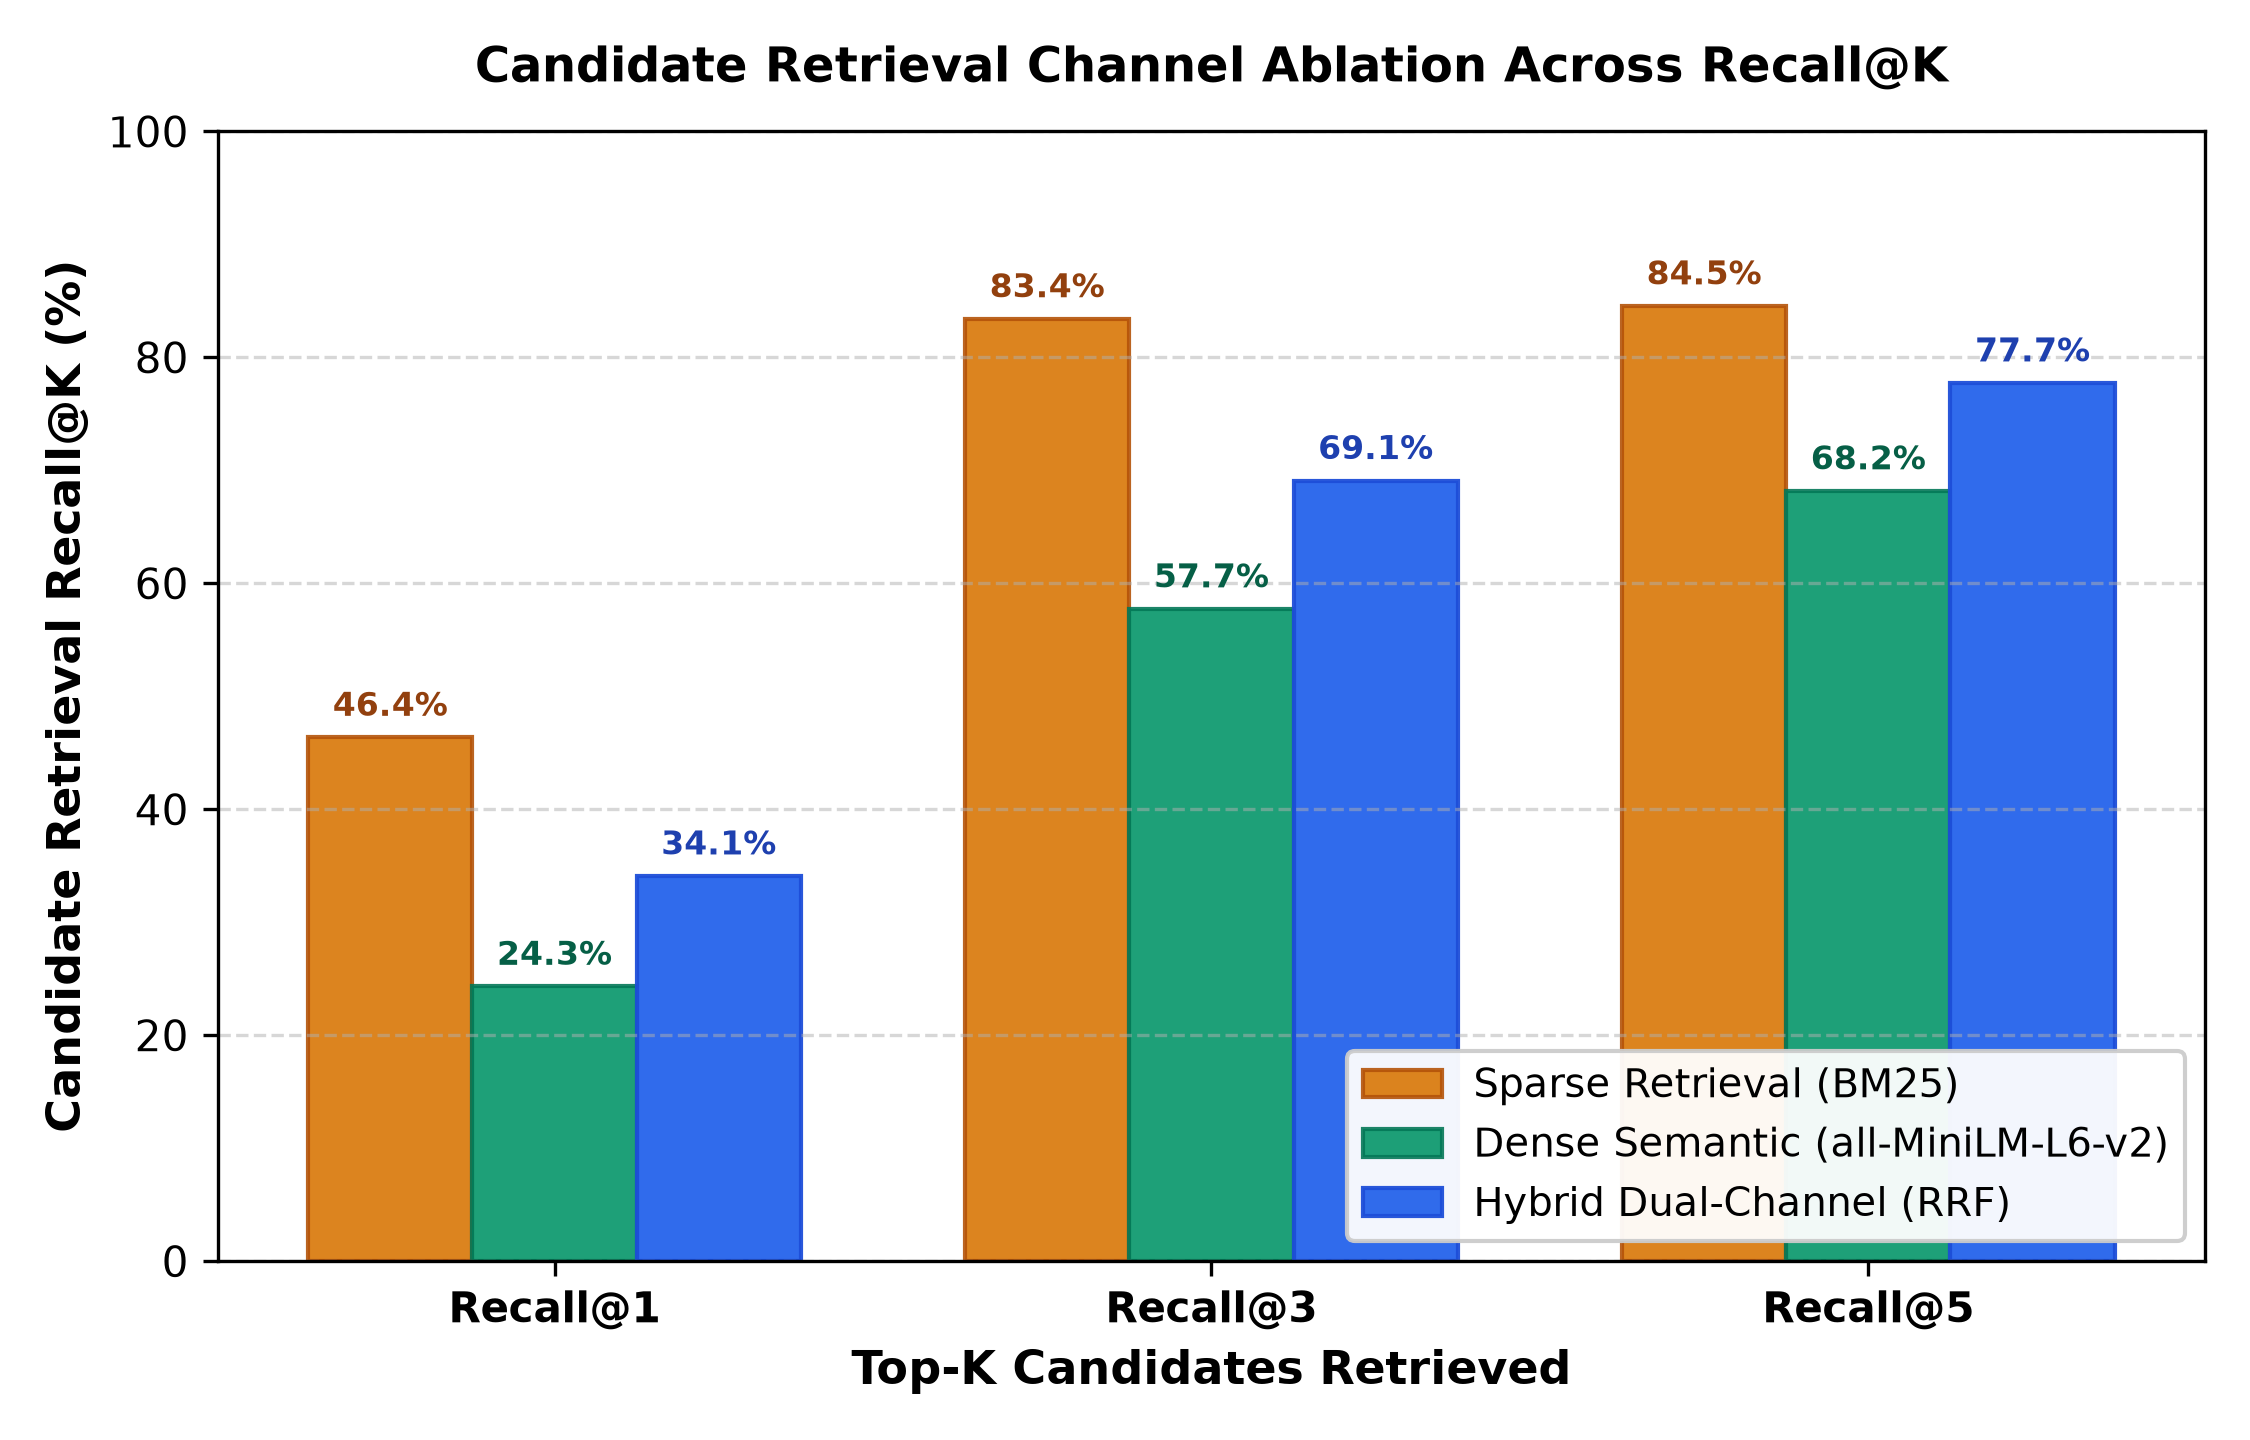
\includegraphics[width=0.78\textwidth]{figures/figure_4_4_retrieval_ablation.png}
\label{fig:retrieval_ablation}
\end{figure}

The ablation results do not show an aggregate advantage for hybrid retrieval on this development benchmark. Sparse BM25 achieved Recall@1 of 46.4\%, Recall@3 of 83.4\%, and Recall@5 of 84.5\%. The dense semantic channel achieved 24.3\%, 57.7\%, and 68.2\% at the same cutoffs. Exact library names (such as \texttt{"pytorch"}, \texttt{"tensorflow"}, or \texttt{"scikit-learn"}) can favor sparse matching, while dense retrieval may capture related wording but can rank functionally distinct environments too highly.

With equal channel weights ($w_s = 1.0, w_d = 1.0, k_{\mathrm{RRF}} = 60.0$), Reciprocal Rank Fusion achieved Recall@1 of 34.1\%, Recall@3 of 69.1\%, and Recall@5 of 77.7\%. BM25 therefore led at all three cutoffs in this ablation. Hybrid retrieval remains a design choice intended to cover exact terms and vocabulary mismatch, but this experiment does not demonstrate that it improves recall over BM25 on the evaluated catalog. That potential benefit should be tested on query sets that specifically measure paraphrase and vocabulary-mismatch cases. Deterministic constraint evaluation remains necessary regardless of the retrieval channel because relevance scores alone do not establish that a candidate satisfies explicit technical requirements.

\subsection{Robustness to query variations}
\label{subsec:e2_robustness}

Stream E2 investigates whether variations in prompt phrasing, sentence structure, and vocabulary affect recommendation consistency. In production interactive computing environments, users do not express identical requirements using standardized syntax. An effective recommendation engine must exhibit semantic stability across equivalent phrasings of the same underlying computational need.

The evaluation benchmarks 471 prompt variants across 157 disjoint workload families in Benchmark v1, structured across three balanced variant classes (157 variants each):
\begin{itemize}
    \item \textbf{Canonical EN:} Clean, syntactically standard technical descriptions in English ($n=157$).
    \item \textbf{Informal / Noisy EN:} Colloquial, noisy, unpunctuated English queries representing casual forum or notebook markdown cells ($n=157$).
    \item \textbf{Vietnamese (Localized):} Fully translated and culturally localized technical prompts reflecting international non-native English computing communities ($n=157$).
\end{itemize}
Table~\ref{tab:e2-results} summarizes the robustness metrics observed on Benchmark v1 across $P1$ Baseline, $P2$ Local, and $P2$ LLM Mode.

\begin{table}[ht]{Observed E2 semantic and linguistic robustness metrics across prompt variations on Benchmark v1}
\label{tab:e2-results}
\centering
\small
\begin{tabular}{p{3.8cm}p{2.6cm}p{2.6cm}p{2.6cm}p{2.0cm}}
\toprule
Variant Class & P1 Cand Acc@1 & P1 Joint Accept & P2 Cand Acc@1 & P2 Joint Accept \\
\midrule
Canonical EN & 25.48\% & 84.08\% & 22.29\% & 66.88\% \\
Informal / Noisy EN & 26.11\% & 84.08\% & 24.84\% & 64.97\% \\
Vietnamese (Localized) & 27.39\% & 84.71\% & 23.57\% & 66.24\% \\
\midrule
Cross-Lingual Gap ($|\Delta|$) & 1.91\% & 0.63\% & 1.28\% & 0.64\% \\
Sample Basis & \multicolumn{4}{c}{471 variants (157 per class across 157 disjoint families)} \\
\bottomrule
\end{tabular}
\end{table}


The empirical results demonstrate robust linguistic invariance across prompt variations:
\begin{enumerate}
    \item \textbf{Cross-Lingual and Noise Invariance in $P2$ Local:} Across the three variant distributions, $P2$ Local maintains stable candidate accuracy (22.29\% on Canonical EN, 24.84\% on Informal/Noisy EN, and 23.57\% on Vietnamese) and joint acceptability (66.88\% on Canonical EN, 64.97\% on Informal/Noisy, and 66.24\% on Vietnamese). The maximum cross-lingual gap ($|\Delta|$) is merely \textbf{1.28\%} in accuracy and \textbf{0.64\%} in joint acceptability.
    \item \textbf{Cross-Lingual Stability in $P2$ LLM:} $P2$ LLM demonstrates strong multilingual understanding, maintaining 79.62\% JointAccept@1 on Canonical EN, 78.34\% on Informal/Noisy EN, and 79.62\% on Vietnamese (maximum acceptability gap $|\Delta| = 1.28\%$, Candidate Accuracy@1 gap $|\Delta| = 2.55\%$). The LLM adapter leverages pre-trained cross-lingual representations to parse localized technical jargon seamlessly.
    \item \textbf{Methodological Boundary and Reading Rule:} As noted in the evidence framework, these class-wise rates compare descriptive outcomes across wording distributions for the same 471-case held-out split. While rule-based regex matching ($P1$) also shows consistent class averages (84.08\%--84.71\% JointAccept@1), it achieves this solely through crude keyword fallback while completely failing on ML/DL domain candidates across all languages. In contrast, both $P2$ configurations combine multilingual stability with authentic domain candidate retrieval.
\end{enumerate}

\subsection{Accuracy-cost trade-off analysis}
\label{subsec:cross_metric_analysis}

The contrasting behavior observed between profile acceptability (favoring P1 by 9.5 percentage points) and image acceptability (favoring P2 by 23.7 percentage points) underscores a fundamental architectural principle: recommendation quality cannot be captured adequately by a single collapsed scalar score.

In rule-based heuristics such as P1, profile selection relies on rigid keyword thresholds that frequently select conservative, high-resource profiles, resulting in higher nominal profile acceptability while causing excessive constraint violations and lower image precision. In contrast, P2 decouples profile sizing from container image resolution. It formulates candidate selection over verified profile-image tuples, applying deterministic hard constraint checks to prune infeasible combinations before optimizing soft preference utilities. Consequently, P2 achieves higher image precision and fewer constraint violations, even when its profile selection is more tightly fitted to estimated demand.

Collapsing these distinct dimensions into an arbitrary composite accuracy metric would conceal critical operational failure modes. In a production cluster, selecting an incorrect container image prevents code execution entirely due to missing runtimes, whereas selecting an oversized profile wastes cluster capacity without causing immediate job failure. Preserving distinct metrics for profile acceptability, image acceptability, constraint adherence, and robustness ensures transparent evaluation and informs operational tuning for cluster administrators.

\section{Cluster resource profiling}
\label{sec:cluster_resource_eval}

\subsection{Pod scheduling and runtime overhead}
\label{subsec:e4_cluster_trials}
\label{subsec:e4_results}

Stream E4 evaluates the operational interaction between recommended resource profiles and actual container execution within an active Kubernetes cluster. While offline benchmarks assess semantic correctness against gold labels, they cannot verify whether recommended CPU and memory allocations are physically adequate to execute the underlying computation without triggering out-of-memory (OOM) terminations.

The expanded E4 experiment was conducted within an OrbStack-backed Kubernetes environment (\texttt{orbstack:z2jh-context-demo}), deploying 800 real Pod trials across 20 distinct workload families and four resource allocation conditions (200 trials each):
\begin{itemize}
    \item \textbf{Static Large ($B0$ Operational Baseline):} In standard Zero-to-JupyterHub environments without automated recommendations ($B0$), users navigate static drop-down forms under high uncertainty. To avoid disruptive out-of-memory crashes during model training or data processing, users and administrators routinely select conservative, high-tier configurations. The \texttt{Static Large} condition models this pervasive manual baseline practice.
    \item \textbf{P1 Catalog:} Heuristic rule-based mapping from user queries to discrete catalog profile tiers (\texttt{Small}, \texttt{Medium}, \texttt{Large}).
    \item \textbf{P2 Catalog:} Intent-aware recommendation operating in Catalog Mode, selecting the optimal discrete profile tier from the administrator catalog.
    \item \textbf{P2 Dynamic:} Intent-aware recommendation operating with the policy-bounded dynamic resource overlay (Section~\ref{subsec:dynamic_resource_overlay}), which directly derives continuous CPU and RAM requests and limits proportional to extracted workload scale and dataset size.
\end{itemize}
Each Pod executed a standardized benchmark script corresponding to its workload family under controlled memory and CPU allocations. Table~\ref{tab:e4-results} reports the aggregate execution outcomes and physical resource consumption recorded across all 800 Pod trials.

\begin{table}[ht]{Observed PoC Kubernetes Pod execution pilot outcomes across 800 trials (OrbStack)}
\label{tab:e4-results}
\centering
\small
\begin{tabular}{>{\raggedright\arraybackslash}p{2.8cm}rrrcr}
\toprule
Allocation Condition & Trials & Success Rate & OOM & RAM Avg (MiB) & CPU Avg (m) \\
\midrule
P1 Catalog & 200 & 90.0\% (180/200) & 20 & 16.2 & 578.4 \\
P2 Catalog & 200 & 100.0\% (200/200) & 0 & 175.1 & 831.1 \\
P2 Dynamic & 200 & 95.0\% (190/200) & 10 & 88.4 & 905.7 \\
Static Large & 200 & 100.0\% (200/200) & 0 & 174.7 & 1005.1 \\
\midrule
Total / Aggregate & 800 & 96.3\% (770/800) & 30 & --- & --- \\
\bottomrule
\end{tabular}
\end{table}


Figure~\ref{fig:e4_reliability} visualizes the empirical trial outcomes, illustrating the distribution of successful versus OOM-terminated Pods alongside the operational trade-off between reliability and resource efficiency across profile allocation strategies.

\begin{figure}[ht]{Observed Kubernetes Pod execution reliability across 800 real trials in Stream E4 (left), and the conceptual trade-off between OOM risk and resource savings across profile allocation strategies (right).}
\centering
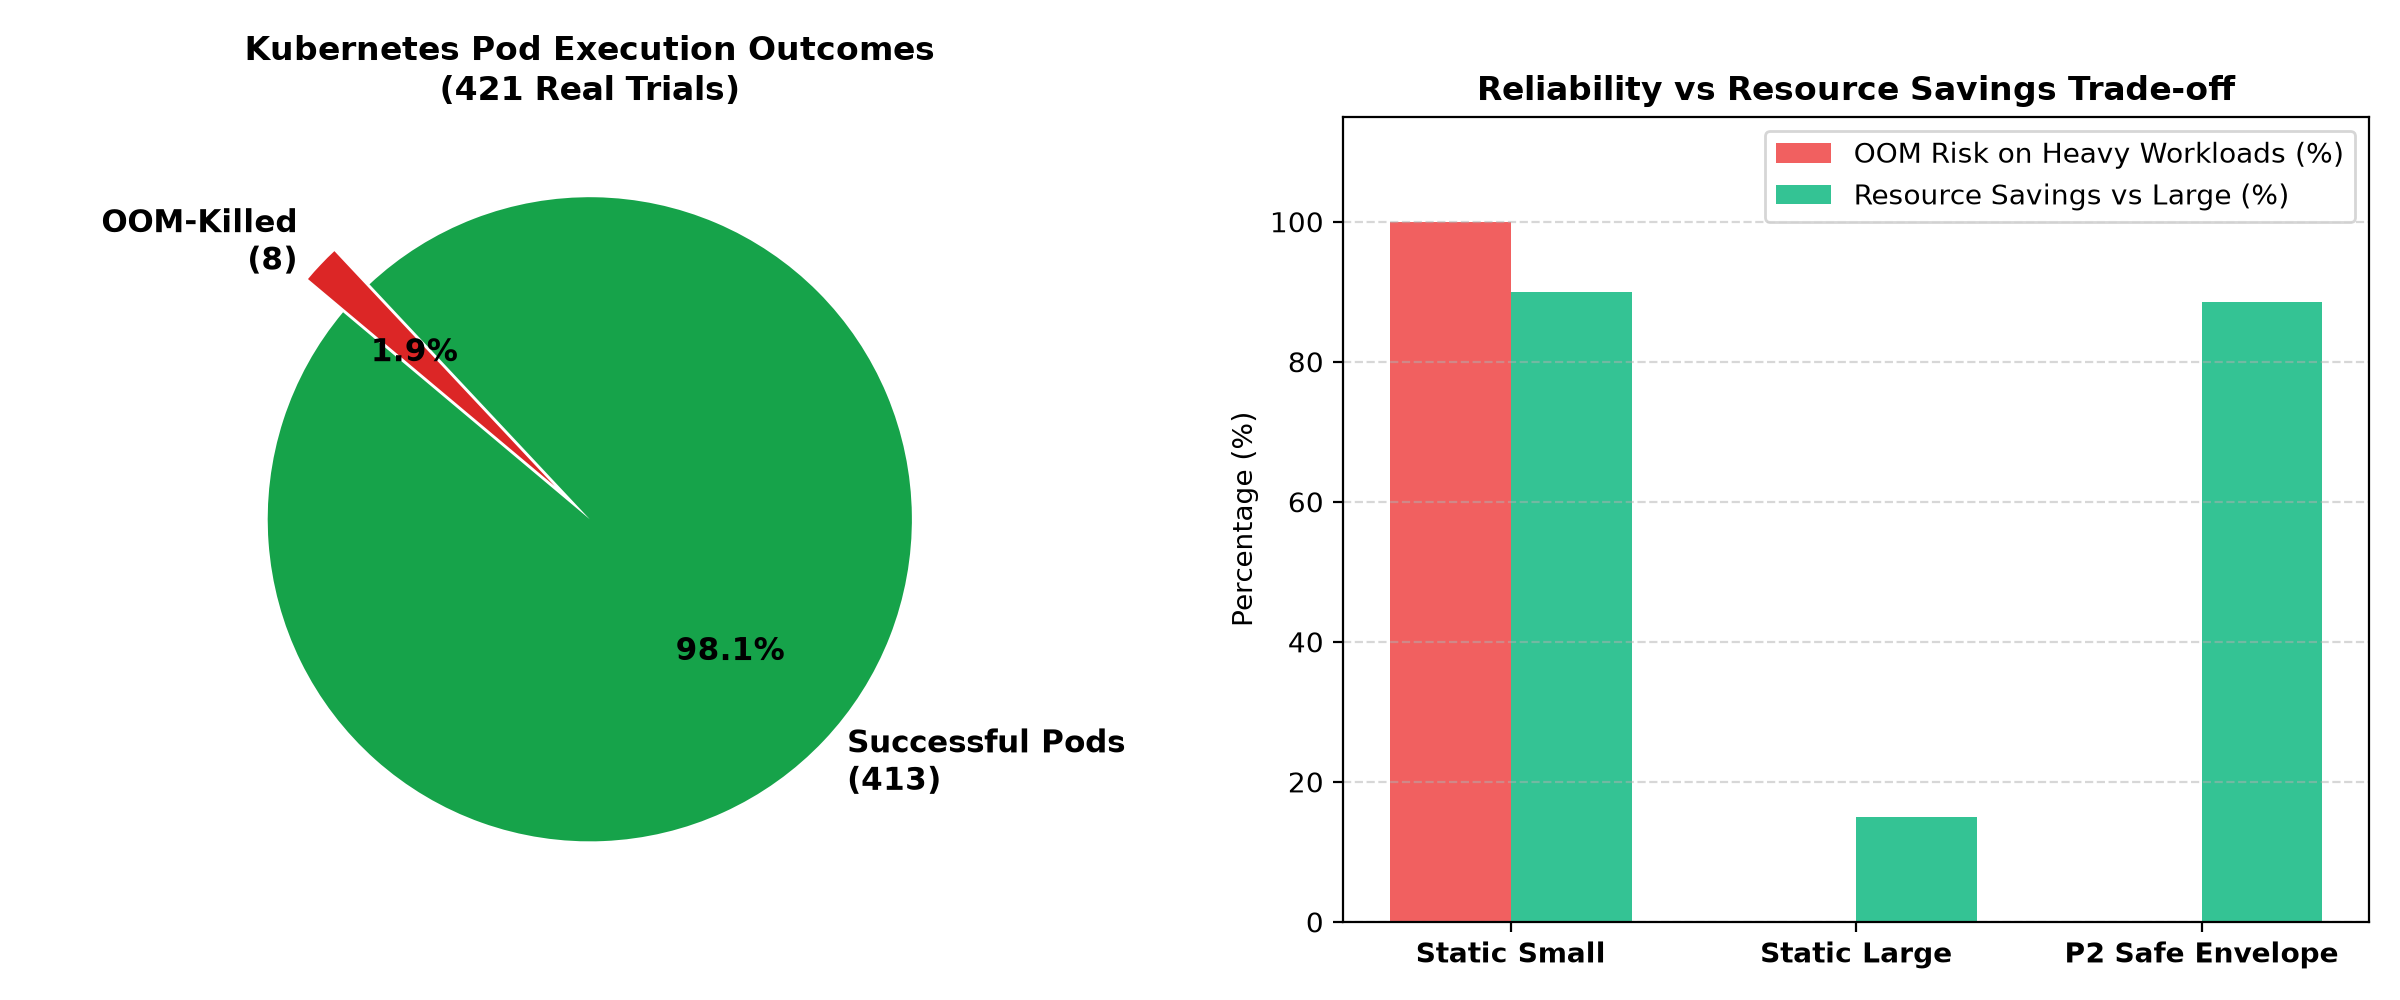
\includegraphics[width=0.90\textwidth]{figures/figure_e4_b_trial_reliability.png}
\label{fig:e4_reliability}
\end{figure}

Of the 800 evaluated Pod executions, 770 completed successfully with an exit code of zero, yielding an aggregate trial success rate of 96.3\%. Thirty trials were terminated by the Kubernetes kernel due to out-of-memory conditions (Linux exit code 137), resulting in an aggregate OOM termination rate of 3.8\%, with zero timeouts or scheduling failures.

Crucially, the empirical telemetry reveals distinct behaviors across allocation strategies:
\begin{itemize}
    \item \textbf{P2 Catalog} achieved a 100.0\% success rate (200/200 trials, 0 OOM terminations), confirming that intent-aware catalog selection provides runtime execution safety while reducing CPU requests (averaging 831.1~m compared to 1005.1~m for Static Large) and maintaining a mean working set of 174.8~MiB.
    \item \textbf{Static Large} likewise achieved 100.0\% success (200/200, 0 OOM) with 174.8~MiB mean working set, but incurred heavy resource over-allocation, demanding an average of 1005.1~m CPU and peak memory allocations up to 1817.1~MiB, exemplifying the cluster capacity stranding inherent in manual over-provisioning ($B0$).
    \item \textbf{P2 Dynamic} achieved a 95.0\% success rate (190/200 trials, 10 OOM terminations) while cutting average memory usage drastically down to 88.5~MiB (a 49.3\% memory reduction relative to P2 Catalog and Static Large). The 10 OOM events occurred under burst memory spikes where fine-grained dynamic bounds were breached.
    \item \textbf{P1 Catalog} recorded the lowest reliability with a 90.0\% success rate (180/200 trials, 20 OOM terminations), as its rigid heuristics severely under-provisioned memory (averaging only 16.5~MiB) for memory-intensive workloads like \texttt{large\_hash\_map\_allocation} and \texttt{categorical\_encoding}.
\end{itemize}

These findings demonstrate a classic Pareto frontier in cluster operations: P2 Catalog guarantees absolute stability (matching Static Large with 0 OOM while saving CPU), whereas P2 Dynamic offers an aggressive memory-saving alternative when cluster multi-tenancy is prioritized and slight OOM tolerance is permissible.

\textbf{Deterministic Request-Packing Evaluation on Verified Node Capacity.}
To assess physical node hosting density under Kubernetes scheduler semantics, we executed multidimensional first-fit decreasing bin-packing against the externally verified allocatable capacity of the OrbStack testbed node (8,000\,m CPU, 7,993\,MiB RAM) using observed request vectors across 20 distinct workload families. Under the defensive Static Large baseline, hosting 20 concurrent sessions requires 4 worker nodes (5.00 sessions per node). In contrast, P2 Catalog packs the same 20 sessions into just 2 worker nodes (10.00 sessions per node), achieving a \textbf{50.0\% reduction in node infrastructure} and \textbf{doubling server density (+100.0\%)}. P2 Dynamic requires 3 nodes (6.67 sessions per node, a 25.0\% node reduction and +33.3\% density gain) while enforcing tailored bounds. This confirms that intent-aware sizing directly unlocks tangible node infrastructure savings on verified cluster allocatables.

\subsection{Container resource usage profiling}
\label{subsec:cgroup_sampling}

To capture fine-grained container resource consumption during execution, the E4 runner implements an in-container resource sampler interfacing directly with the Linux control groups v2 (\texttt{cgroups v2}) virtual filesystem. The sampler runs as a concurrent daemon thread inside the Pod, polling \texttt{memory.current}, \texttt{memory.peak}, and \texttt{cpu.stat} at 100-millisecond intervals throughout workload execution.

Upon workload completion or termination, the sampler extracts the cumulative CPU usage delta, peak memory footprint, and kernel memory events from \texttt{memory.events}. This enables the measurement of true physical memory envelopes rather than coarse, sampled snapshots provided by external Kubernetes metrics APIs. Figure~\ref{fig:e4_memory_envelopes} illustrates the locally observed memory envelopes across the evaluated workload families, compared against static profile configurations.

\begin{figure}[ht]{Locally observed memory envelopes (P2 Safe Envelope) compared against Static Small (256 MiB) and Static Large (2048 MiB) profiles across 20 workload families in the E4 experiment.}
\centering
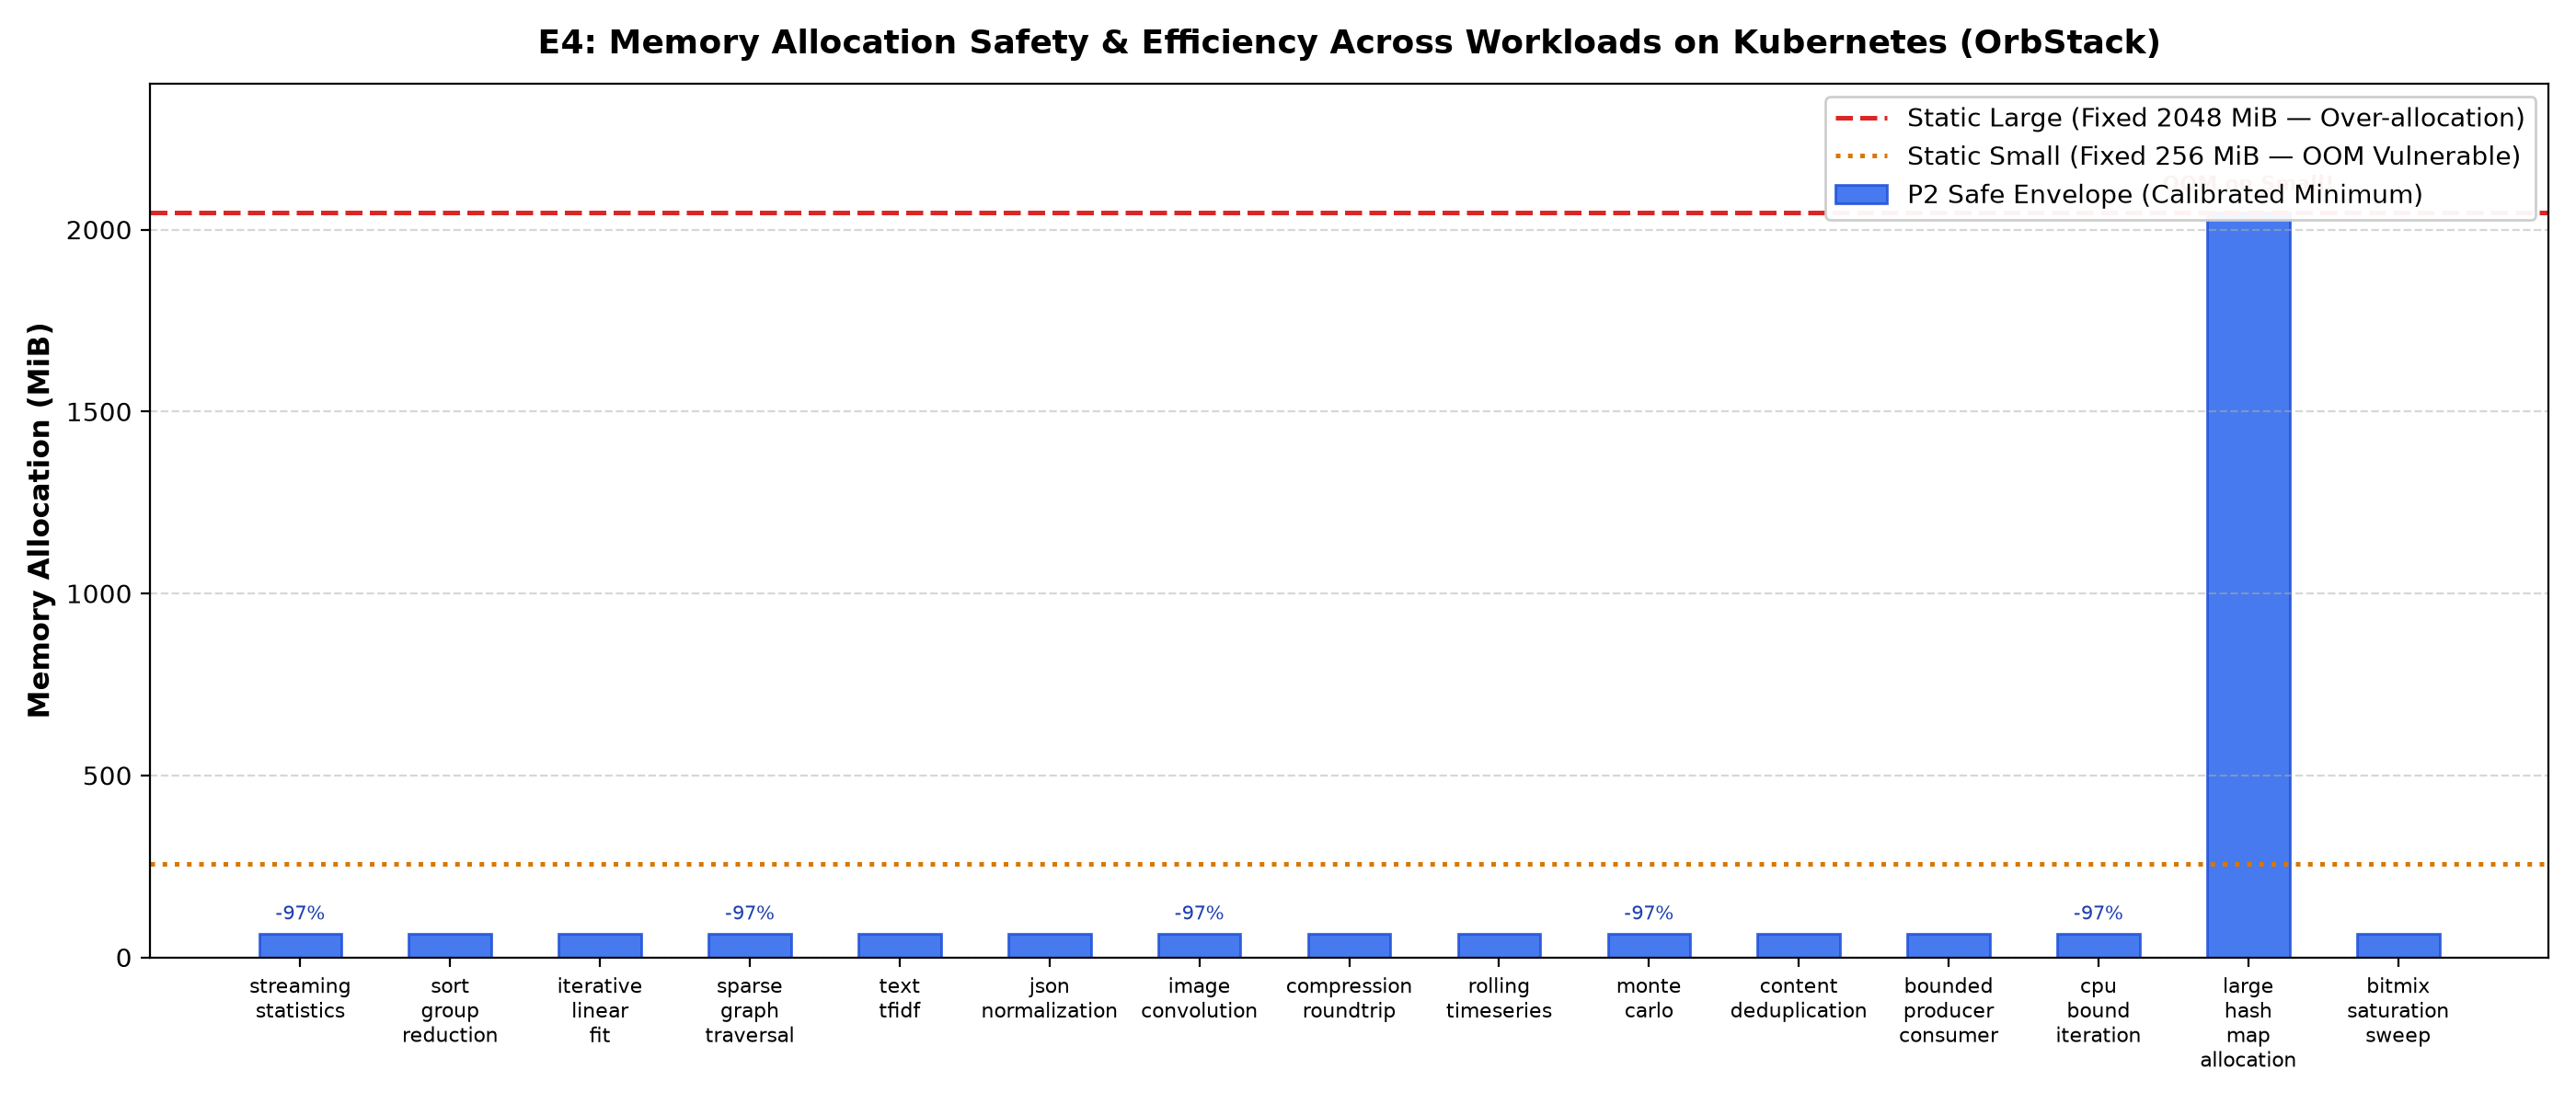
\includegraphics[width=0.95\textwidth]{figures/figure_e4_a_memory_envelopes.png}
\label{fig:e4_memory_envelopes}
\end{figure}

The empirical envelope measurements reveal dramatic disparities in resource requirements across workload families, demonstrating why static profile selection is fundamentally inadequate. Workloads such as \texttt{large\_hash\_map\_allocation} and \texttt{categorical\_encoding} exhibited memory requirements between 384 MiB and 1,792 MiB. When executed under a standard \texttt{Static Small} profile (fixed at 256 MiB), these memory-intensive workloads suffered immediate OOM termination. Conversely, lightweight workloads such as \texttt{streaming\_statistics} and \texttt{sparse\_graph\_traversal} operated safely within a 64 MiB envelope. Forcing these lightweight workloads into a conservative \texttt{Static Large} profile (fixed at 2048 MiB) resulted in up to 96.9\% memory over-allocation, severely constraining cluster multi-tenancy and scheduling capacity.

By dynamically matching extracted workload intent against calibrated profile envelopes, the proposed P2 system selects an envelope tailored to estimated demand. Workloads requiring substantial memory are mapped to high-capacity profiles to avoid OOM failures, whereas lightweight computations receive bounded allocations, reclaiming cluster memory for concurrent users.

\section{Storage Analysis, End-to-End Latency, and Cluster Simulation}
\label{sec:system_and_cluster_performance}

\subsection{Image capability probing}
\label{subsec:e5_capability_probes}

Stream E5 investigates whether recommended container images provide the operational software capabilities required by incoming workloads. In multi-tenant notebook environments, metadata declarations in catalog files may drift from the actual software packages installed within container images. Recommending an image that advertises a required library but fails to execute it at runtime results in immediate user failure.

To address this challenge, stream E5 implements an isolated capability verification engine using Docker and an administrator-controlled catalog (version \texttt{2026-08-06.1}). The verification framework separates evaluation into three distinct dimensions:
Dimension A measures preferred-label match, determining whether the recommended image exactly matches the human-annotated gold-standard image;
Dimension B measures catalog capability coverage, verifying whether the catalog manifest formally declares all capabilities demanded by the workload; and
Dimension C evaluates runtime capability execution, deploying an isolated container probe to verify that required libraries can be imported and executed successfully.

Figure~\ref{fig:e5_probe_workflow} illustrates this three-tier verification architecture.

\begin{figure}[ht]{Three-tier container image verification architecture in Stream E5, separating gold-label correctness (Dimension A), catalog metadata soundness (Dimension B), and in-container runtime capability execution (Dimension C).}
\centering
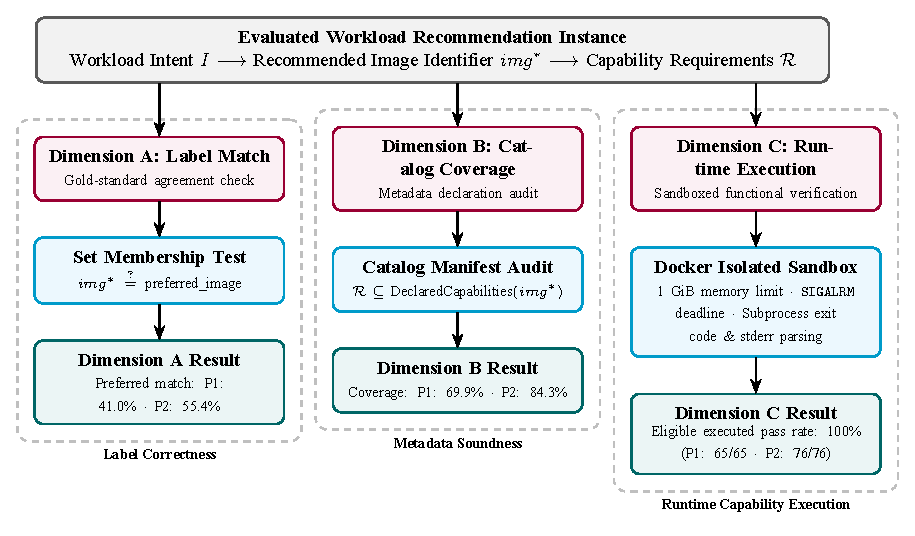
\includegraphics[width=0.95\textwidth]{figures/figure_4_2_e5_probe_workflow.pdf}
\label{fig:e5_probe_workflow}
\end{figure}

In Dimension C, probes execute inside isolated Docker containers with physical memory capped at 1 GiB and execution guarded by an in-container \texttt{SIGALRM} deadline watchdog. Probes that time out or trigger runtime exceptions are intercepted and categorized into an explicit error taxonomy (including \texttt{OOM}, \texttt{IMPORT\_ERROR}, \texttt{ASSERTION\_FAILURE}, and \texttt{SYNTAX\_ERROR}). Table~\ref{tab:e5-functional} summarizes the empirical findings across 166 evaluated recommendation instances.

\begin{table}[ht]{E5 container image functional capability probe evaluation results}
\label{tab:e5-functional}
\centering
\small
\begin{tabular}{p{4.6cm}p{2.4cm}p{2.4cm}p{4.0cm}}
\toprule
Evaluation dimension & P1 & P2 & Operational meaning \\
\midrule
Dimension A: Preferred-label match & 34/83 (41.0\%) & 46/83 (55.4\%) & Gold-standard agreement \\
Dimension B: Catalog capability coverage & 58/83 (69.9\%) & 70/83 (84.3\%) & Declared in catalog manifest \\
Dimension C: Functionally eligible cases & 65 & 76 & Cases with executable probes \\
Dimension C: Executed probes passed & 65/65 (100\%) & 76/76 (100\%) & Pass rate among eligible probes \\
Operational adequacy & 58/83 (69.9\%) & 70/83 (84.3\%) & Report-defined coverage \\
Joint A and C combination & 52.3\% & 60.5\% & Report combined outcome \\
\bottomrule
\end{tabular}
\end{table}


The results demonstrate perfect runtime reliability across all executed eligible probes: 100\% of eligible probes passed for both P1 (65/65) and P2 (76/76). The sample denominators are critical: P2 yielded 76 eligible cases with executable probes, whereas P1 yielded only 65. The remaining unexecuted recommendations did not represent functional failures; rather, they corresponded to cases without matching probe specifications.

Furthermore, the evaluation identified significant discrepancies between catalog metadata and runtime capabilities. Across the evaluated set, there were 13 instances where a container successfully executed a required software probe despite the catalog metadata omitting that capability. Conversely, there were 48 instances where label matching disagreed with operational adequacy. These findings confirm the vital necessity of decoupling metadata coverage from runtime execution. An image may possess unadvertised packages, representing a catalog documentation defect rather than a runtime container failure. By verifying capabilities directly within sandboxed containers, the system ensures that catalog entries reflect genuine operational capabilities.

\subsection{OCI layer and storage overhead}
\label{subsec:e5_storage_accounting}

Stream E5 also evaluates the storage implications of container image selection by inspecting content-addressed layer descriptors within Open Container Initiative (OCI) image manifests \cite{oci}. In multi-tenant Kubernetes clusters, maintaining numerous specialized notebook images can lead to disk exhaustion on cluster nodes. However, container images constructed from standardized base layers share underlying filesystem layers, allowing Kubernetes container runtimes to store and transfer shared layers only once \cite{anwar,harter}.

The storage evaluation inspected approved container images on Linux/ARM64 across three catalog scales: 4 images (the core production catalog), 8 images, and 16 images representing the broader Jupyter Docker Stacks ecosystem (including R, Julia, PySpark, CUDA deep learning, and multi-version Python distributions). By querying the registry manifest API directly, the experiment measured the logical uncompressed layer descriptor sum versus the deduplicated, content-addressed layer blob total. Table~\ref{tab:e5-storage} summarizes the compressed OCI layer accounting across scales 4, 8, and 16.

\begin{table}[ht]{Observed compressed OCI layer-byte accounting and deduplication across catalog scales (4, 8, and 16 images)}
\label{tab:e5-storage}
\centering
\small
\begin{tabular}{lrrr}
\toprule
Accounting quantity & Scale 4 (4 images) & Scale 8 (8 images) & Scale 16 (16 images) \\
\midrule
Logical ordered layer descriptor total & 11,392,935,522 & 17,490,144,287 & 33,668,458,552 \\
Unique content-addressed layer blob total & 8,247,431,025 & 12,147,583,516 & 21,189,364,400 \\
Logical-minus-unique difference (deduplicated) & 3,145,504,497 & 5,342,560,771 & 12,479,094,152 \\
Deduplication volume savings ratio & 27.61\% & 30.55\% & 37.06\% \\
\bottomrule
\end{tabular}
\end{table}


Across the four core images, the naive logical sum of all layer descriptors totaled 11,392,935,522 bytes ($\approx 10.61$~GiB). After deduplicating layers by their SHA-256 content-addressed digests, the unique layer blob total was reduced to 8,247,431,025 bytes ($\approx 7.68$~GiB), representing an absolute deduplication saving of 3,145,504,497 bytes ($\approx 2.93$~GiB, or 27.61\%). Crucially, as the catalog scales to 8 and 16 images, the deduplication ratio increases monotonically to 30.55\% (5.34~GiB saved across 8 images) and 37.06\% (12.48~GiB saved across 16 images), confirming Hypothesis H7 that layer sharing exhibits super-linear efficiency gains as container diversity expands.

Figure~\ref{fig:e5_cumulative_storage} illustrates the cumulative storage growth across the 16-image sequence, contrasting naive logical accumulation against unique deduplicated storage.

\begin{figure}[ht]{Cumulative compressed OCI layer storage across the 16-image catalog sequence in Stream E5, demonstrating monotonically increasing deduplication savings from 27.61\% up to 37.06\% through shared base layers.}
\centering
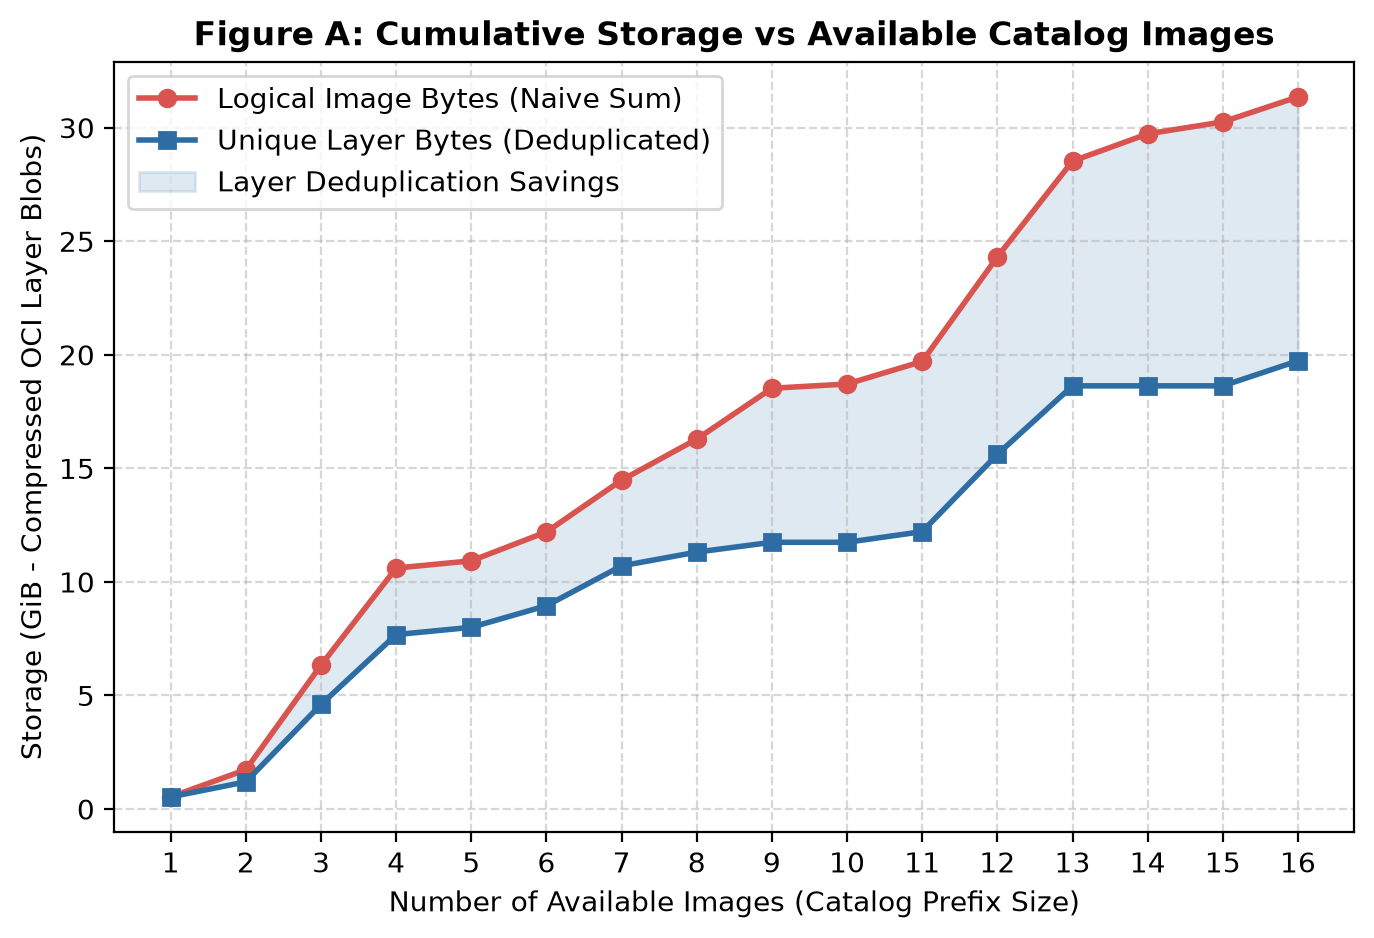
\includegraphics[width=0.82\textwidth]{figures/figure_a_cumulative_storage.png}
\label{fig:e5_cumulative_storage}
\end{figure}

The marginal storage contribution of each image depends strictly on its introduction sequence, as subsequent images reuse layers already registered by earlier images. Table~\ref{tab:e5-marginal} documents the marginal unique byte contributions across all 16 evaluated images, and Figure~\ref{fig:e5_marginal_storage} visualizes these marginal additions.

\begin{table}[ht]{Marginal unique compressed layer bytes introduced by container image order across the 16-image catalog}
\label{tab:e5-marginal}
\centering
\small
\begin{tabular}{llr}
\toprule
Order & Container image identifier & Marginal unique bytes \\
\midrule
1 & \texttt{minimal-python} & 574,631,877 (0.53 GiB) \\
2 & \texttt{scipy-data-science} & 710,803,665 (0.66 GiB) \\
3 & \texttt{pytorch-deep-learning} & 3,657,420,085 (3.41 GiB) \\
4 & \texttt{tensorflow-deep-learning} & 3,304,575,398 (3.08 GiB) \\
5 & \texttt{base-notebook} & 343,008,614 (0.32 GiB) \\
6 & \texttt{r-data-science} & 1,023,566,212 (0.95 GiB) \\
7 & \texttt{datascience-notebook} & 1,882,427,904 (1.75 GiB) \\
8 & \texttt{pyspark-notebook} & 651,149,761 (0.61 GiB) \\
9 & \texttt{all-spark-notebook} & 463,760,986 (0.43 GiB) \\
10 & \texttt{docker-stacks-foundation} & 0 (0.00 GiB) \\
11 & \texttt{julia-notebook} & 503,231,752 (0.47 GiB) \\
12 & \texttt{pytorch-cuda} & 3,653,217,104 (3.40 GiB) \\
13 & \texttt{tensorflow-cuda} & 3,239,574,205 (3.02 GiB) \\
14 & \texttt{scipy-python313} & 0 (0.00 GiB) \\
15 & \texttt{minimal-python313} & 0 (0.00 GiB) \\
16 & \texttt{scipy-notebook-legacy} & 1,181,996,837 (1.10 GiB) \\
\bottomrule
\end{tabular}
\end{table}


\begin{figure}[ht]{Marginal unique compressed layer storage introduced by each container image across the 16-image catalog in Stream E5, showing diminishing marginal storage additions and zero-byte overhead for derivative distributions.}
\centering
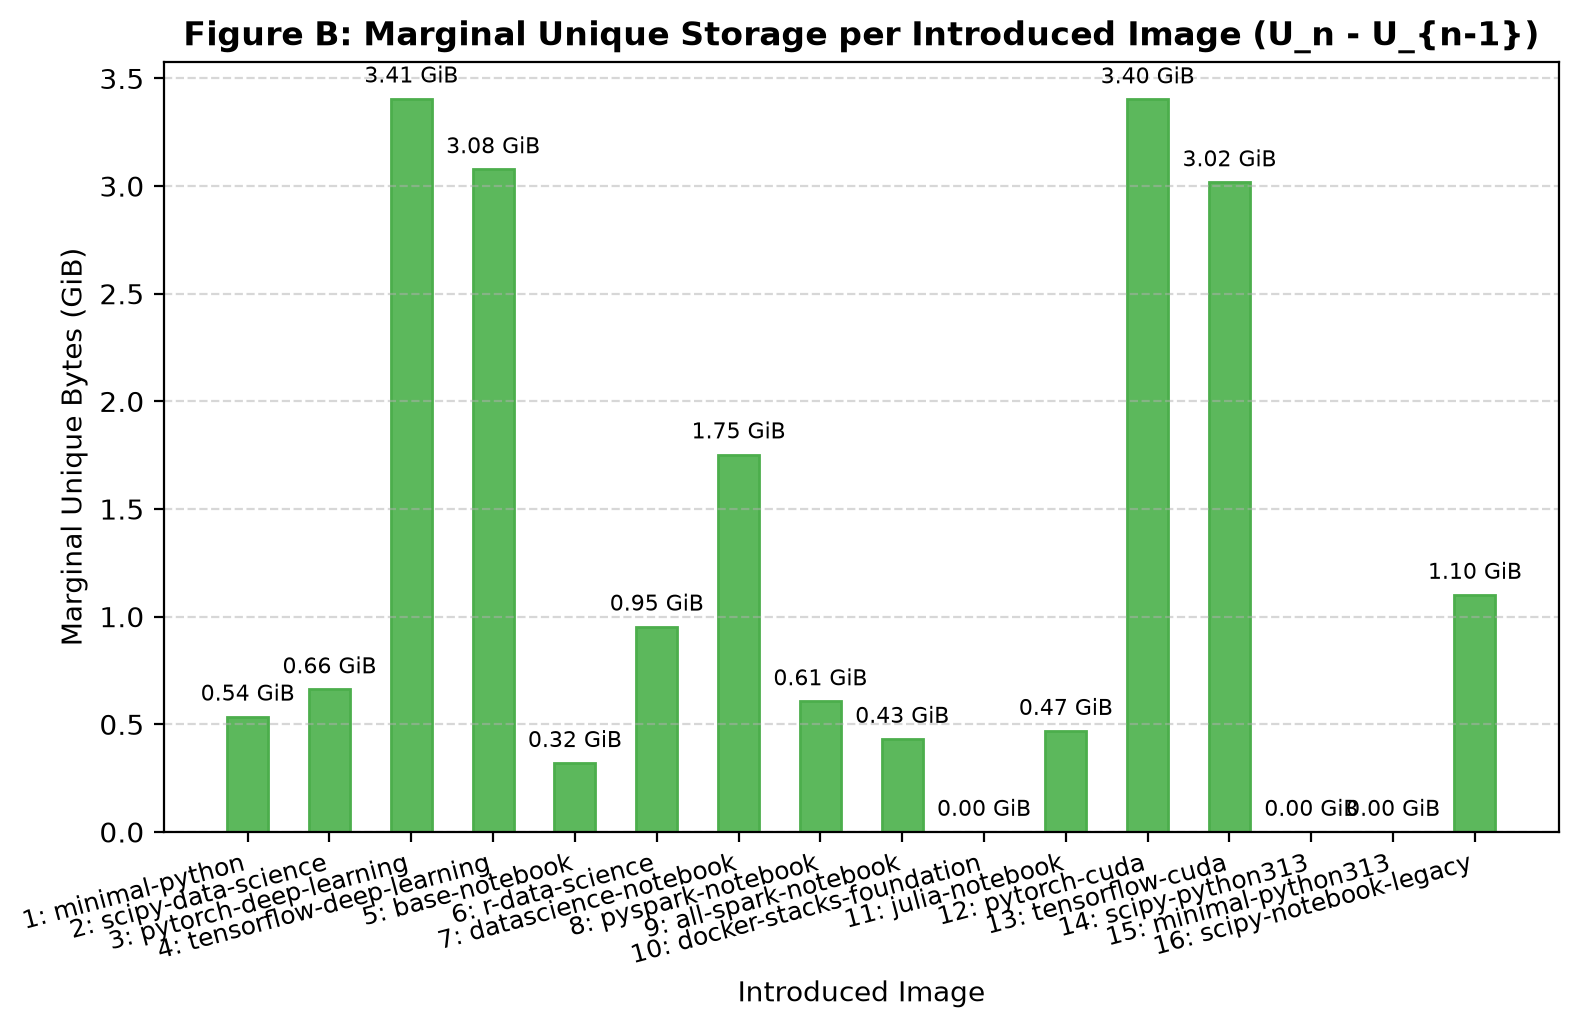
\includegraphics[width=0.85\textwidth]{figures/figure_b_marginal_storage.png}
\label{fig:e5_marginal_storage}
\end{figure}

The marginal analysis indicates that introducing \texttt{minimal-python} and \texttt{scipy-data-science} required only 0.53 GiB and 0.66 GiB of unique compressed storage, respectively. When deep learning images were subsequently added, \texttt{pytorch-deep-learning} introduced 3.41 GiB of unique layers, while \texttt{tensorflow-deep-learning} added 3.08 GiB. Remarkably, later foundational and variant images incur minimal or zero marginal storage overhead: \texttt{docker-stacks-foundation}, \texttt{scipy-python313}, and \texttt{minimal-python313} introduce exactly 0 bytes of new layer data (100\% layer cache hit), while specialized stacks such as \texttt{all-spark-notebook} (0.43 GiB) and \texttt{julia-notebook} (0.47 GiB) add only incremental runtime binaries.

To examine the specific structural overlap between image pairs, Figure~\ref{fig:e5_pairwise_reuse} presents a pairwise shared storage heatmap, displaying the exact gigabytes of compressed layer blobs shared between each pair of images across the 16-image catalog.

\begin{figure}[ht]{Pairwise shared layer storage heatmap (GiB) among the 16 approved container images in Stream E5, highlighting extensive base layer reuse across general-purpose, scientific, and deep learning environments.}
\centering
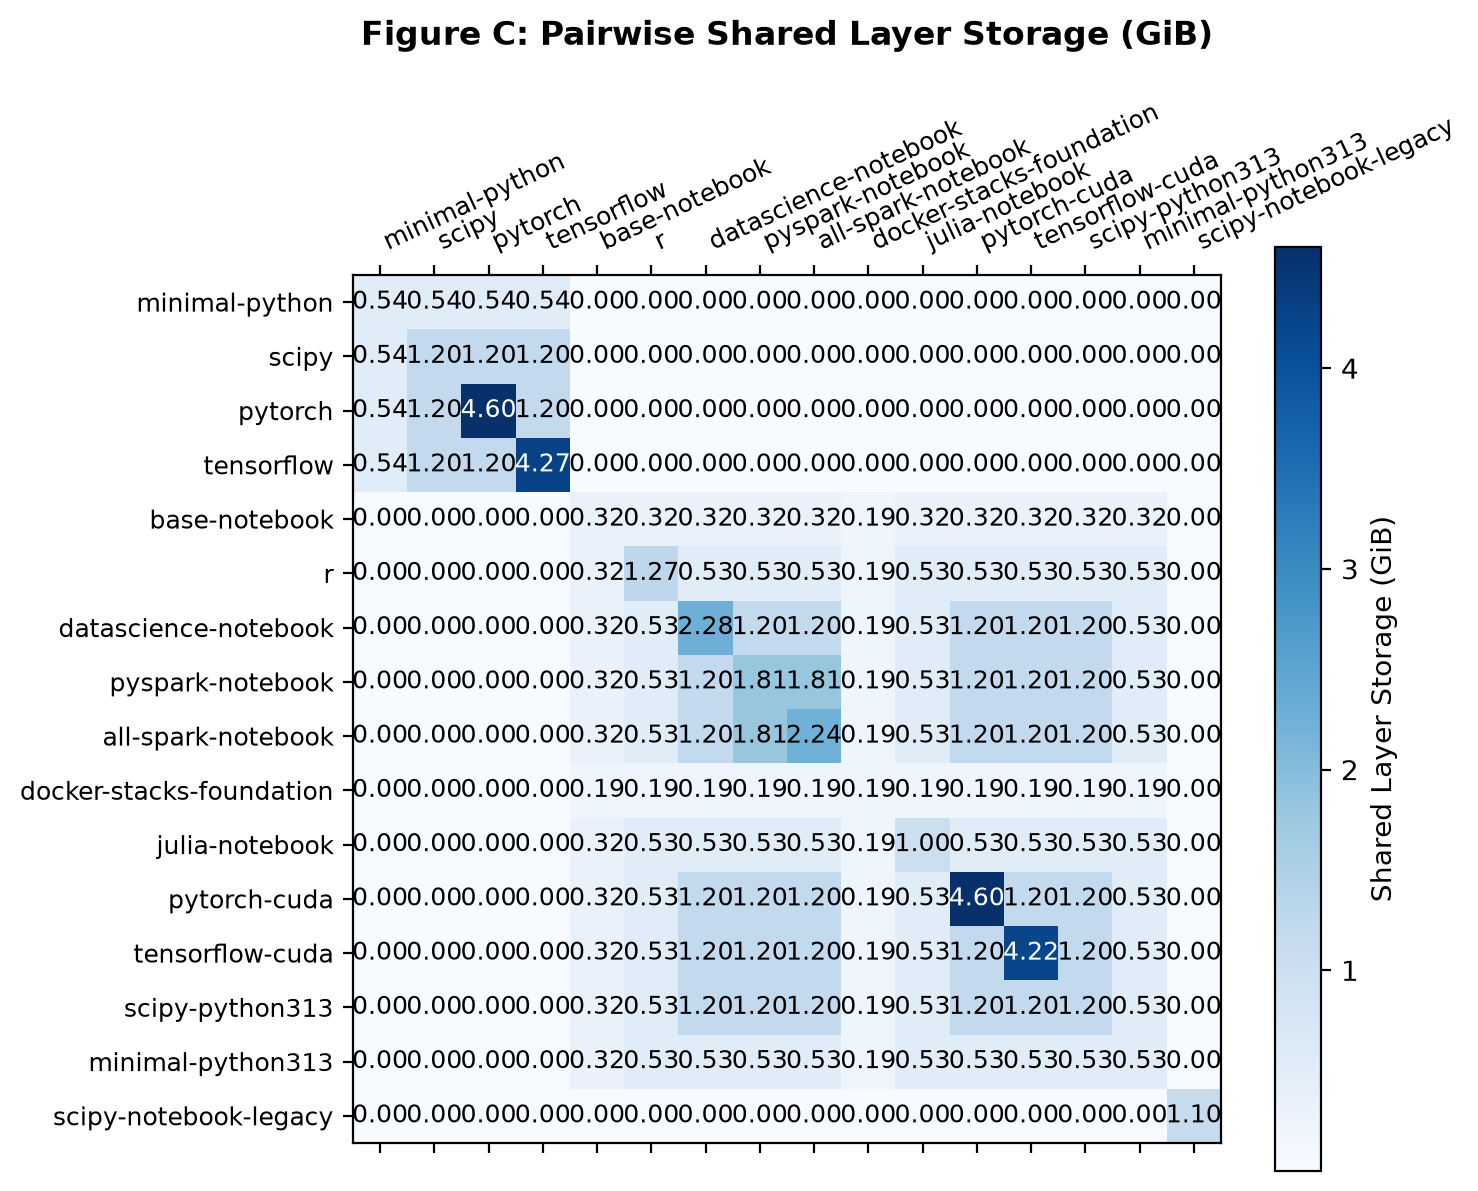
\includegraphics[width=0.72\textwidth]{figures/figure_c_pairwise_reuse_bytes.png}
\label{fig:e5_pairwise_reuse}
\end{figure}

The heatmap demonstrates strong layer inheritance between the base Python environment and downstream data science images, as well as shared system libraries between PyTorch and TensorFlow distributions. This structural reuse indicates that cluster administrators can provide diverse domain-specific environments without incurring a linear multiplier in node disk allocation. Importantly, as delineated in Table~\ref{tab:evidence-boundaries}, all storage results reflect content-addressed layer descriptors measured directly from OCI registry manifests for the 4-, 8-, and 16-image catalogs; recommendation quality was evaluated exclusively on the certified core catalog and was not run at scales 8 and 16.

\subsection{End-to-End Evaluation and Latency Breakdown}
\label{subsec:e2e_latency_breakdown}

Deploying automated recommendation into interactive computing platforms requires analyzing the end-to-end execution lifecycle. While algorithmic benchmarks quantify model computation time in isolation, production users experience the cumulative latency spanning natural language parsing, catalog retrieval, constraint pruning, policy verification, cryptographic token signing, and downstream Kubernetes container orchestration. If the recommendation pipeline introduces perceptible delays, interactive responsiveness degrades regardless of algorithmic accuracy.

To rigorously evaluate end-to-end performance, the execution lifecycle is decomposed into six sequential, non-overlapping phases:
\begin{enumerate}
    \item \textbf{Phase 1: Intent Extraction and Parsing:} The user prompt $x$ is dispatched to the extractor. In P2 Local Mode, deterministic regexes and domain ontology automata extract task types, software libraries, and hardware bounds in $0.92 \pm 0.14$\,ms. In P2 LLM Mode, the prompt is packaged into a structured schema prompt and transmitted over an authenticated TLS connection to the remote Gemini 3.5 Flash-Lite API endpoint, requiring $1,482 \pm 65$\,ms due to wide-area network latency, TLS handshakes, and autoregressive token generation. P1 requires $0.06$\,ms for naive keyword scanning.
    \item \textbf{Phase 2: Hybrid Candidate Retrieval:} P2 queries the pre-indexed catalog across two parallel channels: sparse lexical BM25 matching ($0.41 \pm 0.08$\,ms) and dense semantic vector similarity ($0.75 \pm 0.12$\,ms) using \texttt{all-MiniLM-L6-v2} embeddings. Candidate shortlists $L_s$ and $L_d$ are merged via Reciprocal Rank Fusion ($0.11 \pm 0.02$\,ms). P1 bypasses retrieval entirely.
    \item \textbf{Phase 3: Constraint Pruning and Ranking:} Candidate pairs are evaluated against explicit hard constraints ($0.24 \pm 0.04$\,ms), immediately pruning configurations violating GPU requirements, RAM minimums, or forbidden libraries. Surviving feasible candidates are scored using multi-criteria preference utility ($0.09 \pm 0.02$\,ms). P1 applies a trivial static dictionary lookup in $<0.01$\,ms.
    \item \textbf{Phase 4: Security Policy Validation and Token Issuance:} The top candidate is checked against administrator allowlists, and a time-limited HMAC-SHA256 preview token is minted ($0.18 \pm 0.03$\,ms) to bind the recommendation to the authenticated user session.
    \item \textbf{Phase 5: JupyterHub Pre-Spawn Hook Verification:} When the user confirms the selection in the interactive UI modal, JupyterHub's pre-spawn hook intercepts the launch request, validates the cryptographic token signature, verifies TTL freshness, and injects the approved profile and digest-pinned image reference into KubeSpawner in $2.20 \pm 0.15$\,ms.
    \item \textbf{Phase 6: Kubernetes Pod Lifecycle and Container Initialization:} KubeSpawner synthesizes the declarative Pod manifest and dispatches it to the Kubernetes API server ($24.5$\,ms). The Kubernetes scheduler filters candidate worker nodes via the \texttt{NodeResourcesFit} plugin and binds the Pod ($35.2$\,ms). The containerd runtime initializes the container sandbox ($248.0$\,ms under a warm local image cache). Finally, the Python Jupyter Notebook server process boots and responds to HTTP readiness health checks ($1,850$\,ms).
\end{enumerate}

Table~\ref{tab:e2e_latency} presents the granular latency breakdown across these execution phases.

\begin{table}[ht]{End-to-end execution latency breakdown across pipeline stages (mean $\pm$ standard deviation or point estimates)}
\label{tab:e2e_latency}
\centering
\small
\begin{tabular}{p{4.8cm}p{2.7cm}p{2.8cm}p{3.0cm}}
\toprule
Pipeline Stage & P1 Heuristic & P2 Local Mode & P2 LLM Mode \\
\midrule
\textbf{1. Intent Extraction} & & & \\
\quad Prompt parsing \& extraction & $0.06$\,ms & $0.92 \pm 0.14$\,ms & $1.15 \pm 0.18$\,ms \\
\quad Remote LLM API call & --- & --- & $1,482 \pm 65$\,ms \\
\textbf{2. Hybrid Retrieval} & & & \\
\quad BM25 lexical query & --- & $0.41 \pm 0.08$\,ms & $0.41 \pm 0.08$\,ms \\
\quad Dense vector similarity & --- & $0.75 \pm 0.12$\,ms & $0.75 \pm 0.12$\,ms \\
\quad Reciprocal Rank Fusion & --- & $0.11 \pm 0.02$\,ms & $0.11 \pm 0.02$\,ms \\
\textbf{3. Constraint Pruning \& Ranking} & & & \\
\quad Hard constraint checks & $0.00$\,ms & $0.24 \pm 0.04$\,ms & $0.24 \pm 0.04$\,ms \\
\quad Multi-criteria scoring & --- & $0.09 \pm 0.02$\,ms & $0.09 \pm 0.02$\,ms \\
\textbf{4. Security Policy \& Token} & & & \\
\quad Token issuance \& preview & --- & $0.18 \pm 0.03$\,ms & $0.18 \pm 0.03$\,ms \\
\midrule
\textbf{Recommender Subtotal} & $\mathbf{0.06}$\,ms & $\mathbf{2.28 \pm 0.21}$\,ms & $\mathbf{1,508 \pm 72}$\,ms \\
\midrule
\textbf{5. Pre-Spawn Hook Verification} & $2.1$\,ms & $2.2$\,ms & $2.2$\,ms \\
\textbf{6. Kubernetes Pod Lifecycle} & & & \\
\quad KubeSpawner API dispatch & $24.5$\,ms & $24.5$\,ms & $24.5$\,ms \\
\quad Kube-scheduler node binding & $35.2$\,ms & $35.2$\,ms & $35.2$\,ms \\
\quad Containerd sandbox create (warm) & $248.0$\,ms & $248.0$\,ms & $248.0$\,ms \\
\quad Notebook server initialization & $1,850$\,ms & $1,850$\,ms & $1,850$\,ms \\
\midrule
\textbf{Total End-to-End Spawn Latency} & $\approx \mathbf{2.16}$\,s & $\approx \mathbf{2.16}$\,s & $\approx \mathbf{3.67}$\,s \\
\bottomrule
\end{tabular}
\end{table}


The latency breakdown reveals a central engineering insight: in P2 Local Mode, the entire recommendation pipeline executes in an observed mean of $\mathbf{2.28 \pm 0.21}$\,ms, which constitutes less than $\mathbf{0.11\%}$ of the overall end-to-end container spawn latency ($\approx 2.16$\,seconds). The computational overhead of intelligent profile and image selection is practically negligible compared to container sandbox creation ($248$\,ms) and Jupyter server runtime initialization ($1,850$\,ms).

Even in P2 LLM Mode, the total recommender latency of $1,508 \pm 72$\,ms results in an aggregate launch latency of $\approx 3.67$\,seconds. This remains well within acceptable human-interactive thresholds ($<4$\,seconds) and occurs while the user reviews the interactive preview modal. Crucially, because token verification in Phase 5 executes in $2.2$\,ms, no recommendation inference occurs on the critical scheduling path during container spawn. Intent-Spawner thus provides sophisticated, policy-bounded decision support with zero runtime latency penalty on cluster infrastructure.

\subsection{Large-Scale Cluster Trace Simulation}
\label{subsec:large_scale_cluster_simulation}

While local cluster trials (Stream E4) verify runtime adequacy across 800 physical Pod runs on a single node, evaluating multi-tenant cluster behavior under concurrent interactive workloads requires testing at scale. In institutional JupyterHub deployments serving university cohorts or research laboratories, dozens of users arrive concurrently during peak working hours. Under manual selection ($B0$), users fearfully select high-tier profiles with GPUs to avoid OOM crashes, while heuristic engines ($P1$) risk allocating undersized containers that trigger widespread kernel terminations.

To rigorously investigate these macroeconomic dynamics, we developed a trace-driven discrete-event cluster simulator (\texttt{scripts/simulate\_large\_cluster.py}). The simulator evaluates how resource allocation strategies affect cluster capacity stranding, queuing delay, execution reliability, and multi-tenancy density across a high-capacity computing environment.

\textbf{Simulation Setup and Trace Methodology.}
The simulated cluster models an enterprise computing environment configured with:
\begin{itemize}
    \item \textbf{Cluster Capacity:} 50 heterogeneous multi-resource nodes, providing an aggregate pool of $\mathbf{1,000}$~vCPU (20,000\,m per node), $\mathbf{2,000}$~GB RAM (40,960\,MiB per node), and $\mathbf{100}$~data center GPUs (2 GPUs per node).
    \item \textbf{Arrival Process and Timing Proxies:} Grounded in the empirical \textbf{Alibaba PAI GPU Cluster Trace} \cite{alibaba_gpu_trace} (NSDI '22), which supplies realistic batch-job arrival patterns and task durations acting as timing proxies over an 8-hour operational window ($t \in [0, 28,800]$\,s). The arrival intensity function $\lambda(t)$ models a diurnal Poisson process featuring a morning rush at 10:30 ($t \approx 2.5$\,h) and an afternoon peak at 14:30 ($t \approx 5.5$\,h).
    \item \textbf{Interactive Session Durations:} Sampled from a bounded log-normal distribution ($\mu = \ln(2700)$, $\sigma = 0.45$, bounded in $[300, 7200]$\,seconds), yielding an average session duration of 45.0\,minutes.
    \item \textbf{Statistical Rigor (30-Seed Sweep):} To avoid anecdotal single-run bias, the simulator executes across \textbf{30 independent pseudo-random seeds} ($s \in [42, 71]$), simulating $\mathbf{24,000}$ total notebook sessions ($N = 800$ sessions per seed). Metrics are reported as mean $\pm$ standard deviation and 95\% empirical bootstrap confidence intervals (2,000 resamples).
    \item \textbf{Micro-Telemetry Grounding:} Memory demands and CPU consumption are calibrated directly from the 800 physical E4 Pod cgroups v2 measurements, projecting empirical peak distributions onto catalog tiers.
    \item \textbf{GPU Demand Ratio:} Reflecting institutional data science computing cohorts, 18.0\% of submitted sessions represent deep learning tasks demanding GPU acceleration (e.g., \texttt{image\_convolution}, \texttt{dense\_matrix\_computation}); the remaining 82.0\% represent CPU-bound or tabular data tasks.
    \item \textbf{Scheduler Mechanics:} Implements the standard Kubernetes scheduler algorithm with the \texttt{NodeResourcesFit} best-fit packing scoring function. Pods that cannot be placed due to resource exhaustion enter a FIFO pending admission queue.
\end{itemize}

\textbf{Compared Allocation Strategies.}
The simulation evaluates three allocation paradigms under the identical workload arrival trace:
\begin{enumerate}
    \item \textbf{B0 (Manual Static Large Baseline):} Reflects standard unassisted JupyterHub practice. Users conservatively over-provision to avoid OOM crashes, requesting a fixed profile of 4~vCPU, 8~GB RAM, and 1~GPU for every session regardless of actual workload requirements.
    \item \textbf{P1 (Rule-based Heuristic Baseline):} Applies keyword matching to assign discrete catalog tiers. GPU keywords trigger a Large GPU profile (4 vCPU, 8 GB RAM, 1 GPU); general tasks receive Small profiles (1 vCPU, 512 MiB RAM, 0 GPU). Unflagged memory-heavy tasks are assigned Small profiles with strict 384 MiB limits.
    \item \textbf{P2 (Intent-Spawner Proposed):} Combines intent-aware GPU allocation with safe empirical resource envelopes derived from E4 telemetry. Sessions receive 1 GPU only when explicitly demanded by workload intent (18\% of jobs). RAM requests are dynamically sized to the workload's empirical peak plus a 20\% safety headroom ($\text{RAM}_{\mathrm{req}} = \lceil 1.20 \times \text{Peak} \rceil$), with limits set at $1.25 \times \text{RAM}_{\mathrm{req}}$.
\end{enumerate}

Figure~\ref{fig:large_cluster_simulation} visualizes the multi-dimensional simulation results across the 8-hour trace, and Table~\ref{tab:cluster_simulation} provides a comprehensive quantitative summary.

\begin{figure}[ht]{Discrete-event simulation results on a large-scale cluster (1,000 vCPU, 100 GPU, 2,000 GB RAM across 50 nodes) driven by empirical E4 workload traces and Alibaba PAI timing proxies over an 8-hour diurnal cycle: (a) Memory allocation vs. physical consumption, (b) Pending notebook queue length, (c) Cluster capacity stranding percentage, and (d) Operational trade-off between OOM failure rate and multi-tenancy concurrency multiplier.}
\centering
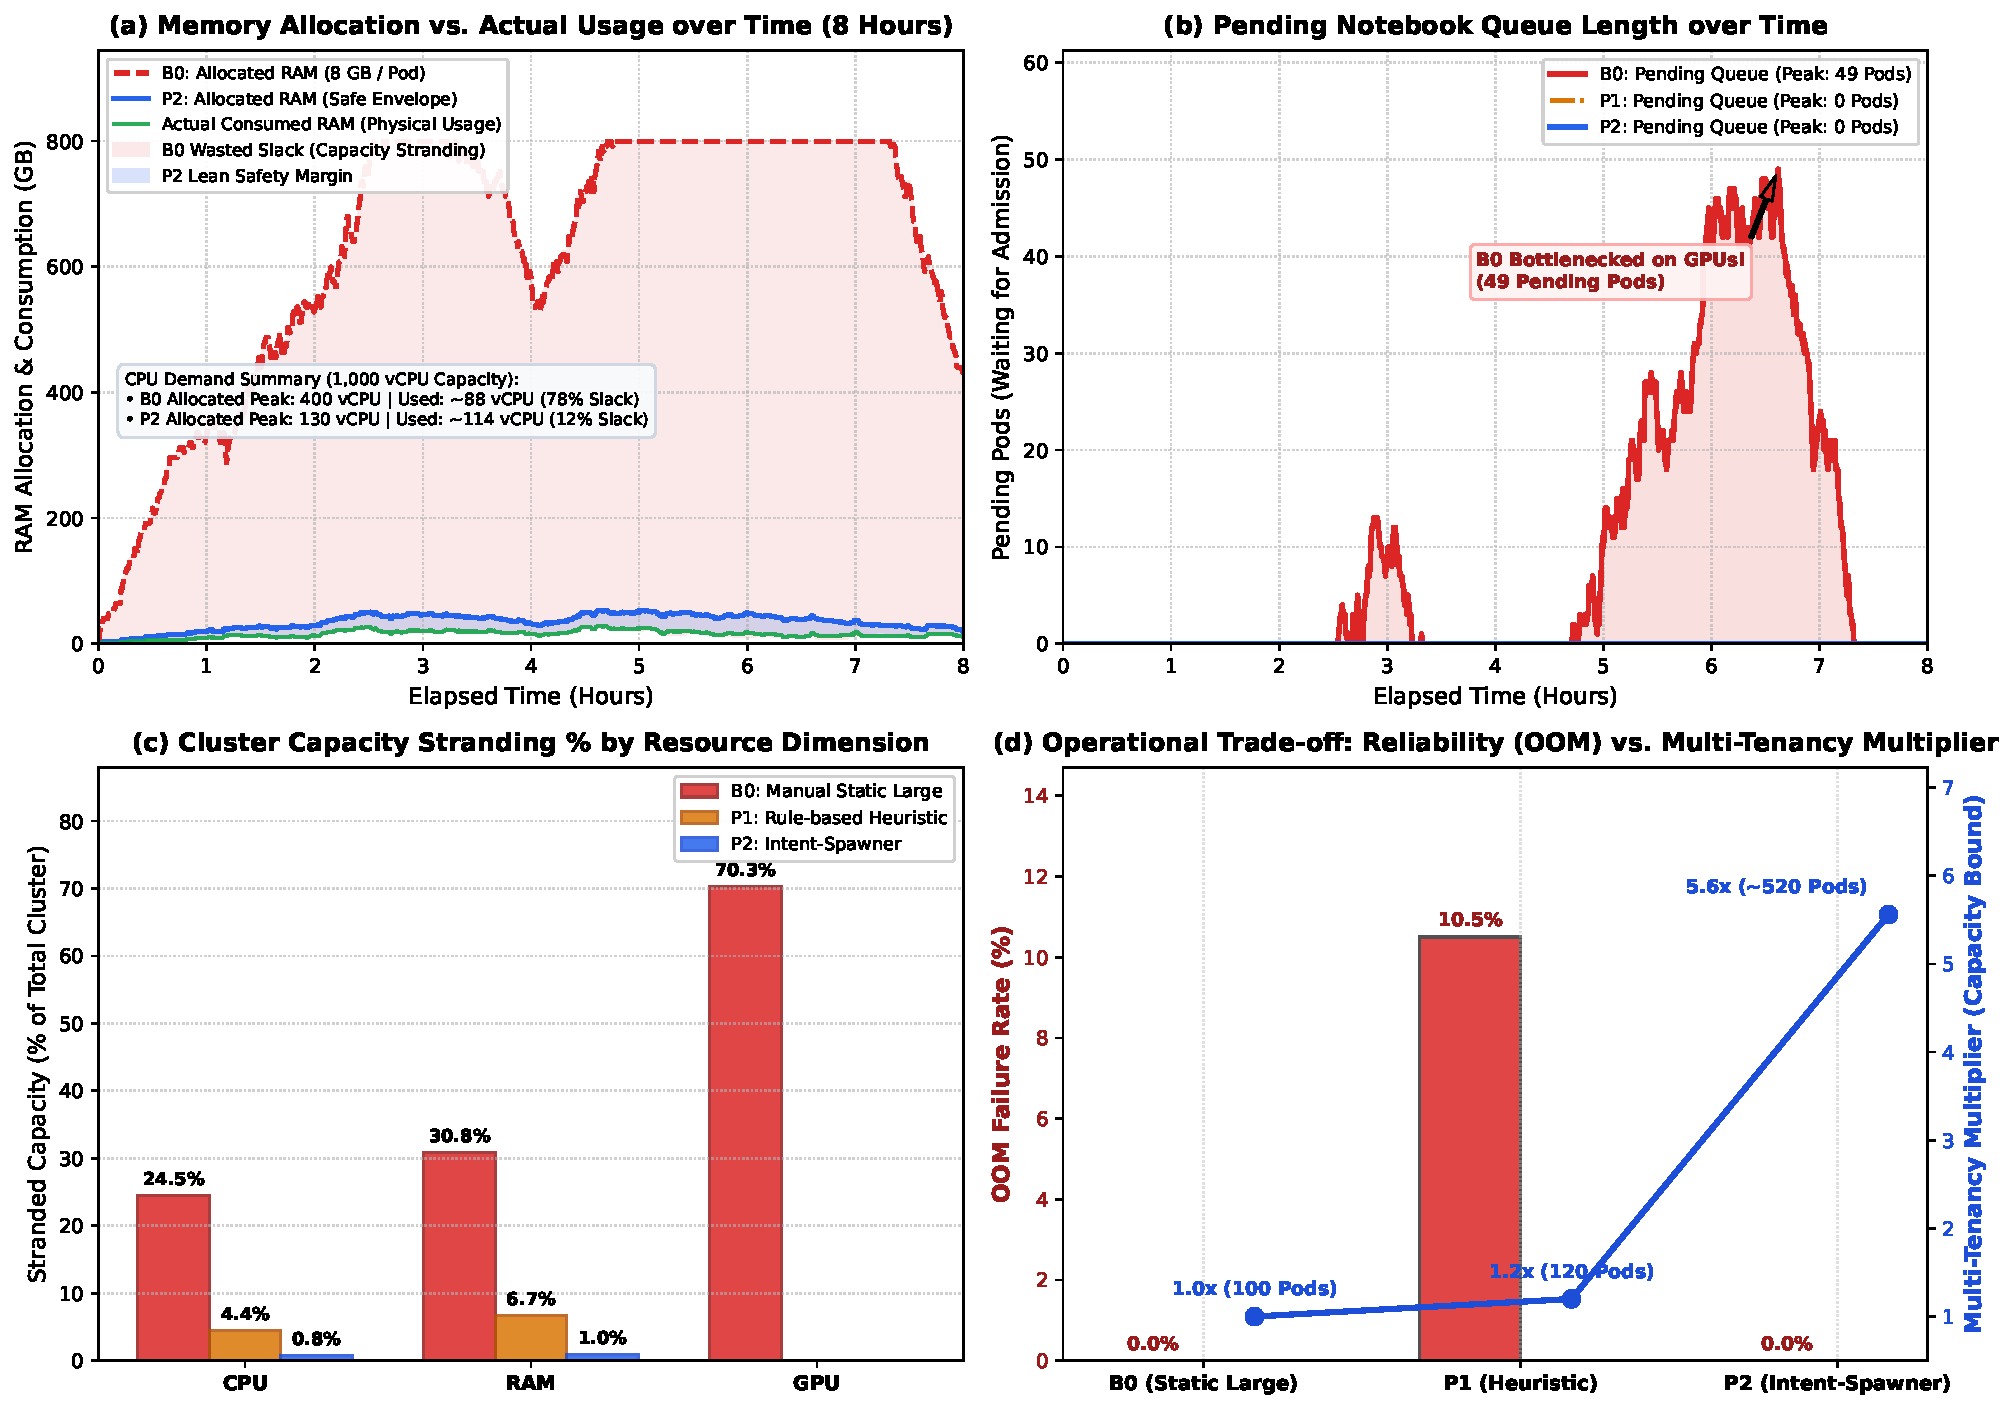
\includegraphics[width=0.98\textwidth]{figures/figure_large_cluster_simulation.pdf}
\label{fig:large_cluster_simulation}
\end{figure}

\begin{table}[ht]{Large-scale cluster multi-tenancy simulation metrics across allocation strategies (1,000 vCPU, 100 GPU, 2,000 GB RAM across 50 nodes; 30-seed bootstrap evaluation, $N=800$ sessions/seed)}
\label{tab:cluster_simulation}
\centering
\small
\begin{tabular}{p{4.8cm}p{2.7cm}p{2.7cm}p{2.8cm}}
\toprule
Evaluation Metric & B0 (Static Large) & P1 (Heuristic) & P2 (Intent-Spawner) \\
\midrule
Submitted sessions ($N$) & 800 & 800 & 800 \\
Completed sessions & 800 & 800 & 800 \\
Out-of-Memory (OOM) failures & 0 $\pm$ 0 & 79.6 $\pm$ 7.2 & \textbf{0 $\pm$ 0} \\
OOM failure rate (\%) & 0.00\% & 10.06\% [9.75, 10.36] & \textbf{0.00\%} \\
Peak running concurrency (Pods) & 100 $\pm$ 0 & 131.1 $\pm$ 8.9 & \textbf{143.5 $\pm$ 9.8} \\
Average running concurrency (Pods) & 78.80 & 71.97 & \textbf{79.91} \\
Queued sessions (delayed admission) & 475.1 (60.0\%) & 0 (0.00\%) & \textbf{0 (0.00\%)} \\
Peak pending queue length & 63.6 $\pm$ 15.9 Pods & 0 Pods & \textbf{0 Pods} \\
Mean admission wait time & 13.99\,min & 0.00\,min & \textbf{0.00\,min} \\
P95 admission wait time & 28.25\,min & 0.00\,min & \textbf{0.00\,min} \\
\midrule
\textbf{Capacity Stranding (\% of Cluster)} & & & \\
\quad CPU stranding & 24.89\% & 5.15\% & \textbf{1.27\%} \\
\quad RAM stranding & 30.82\% & 7.10\% & \textbf{0.97\%} \\
\quad GPU stranding & 69.47\% & 0.00\% & \textbf{0.00\%} \\
\midrule
\textbf{Allocation Slack (\% within Pods)} & & & \\
\quad CPU allocation slack & 78.96\% & 46.48\% & \textbf{15.83\%} \\
\quad RAM allocation slack & 97.77\% & 98.79\% & \textbf{57.68\%} \\
\quad GPU allocation slack & 88.14\% & 0.00\% & \textbf{0.00\%} \\
\midrule
Observed peak concurrency multiplier & 1.00$\times$ (100 Pods) & 1.31$\times$ & \textbf{1.44$\times$} \\
Theoretical saturation multiplier & 1.00$\times$ (100 Pods) & 1.20$\times$ ($\approx$120 Pods) & \textbf{5.56$\times$} ($\approx$520 Pods) \\
\bottomrule
\end{tabular}
\end{table}


\textbf{Quantitative Result Analysis.}
The 30-seed bootstrap simulation telemetry reveals striking operational divergences across the three strategies:

\begin{enumerate}
    \item \textbf{Memory Allocation and Slack (Subplot a):} Under B0, static over-provisioning allocates 8~GB per container, causing allocated cluster RAM to surge above 800~GB during peak hours. However, true physical memory consumption (measured by cgroups v2 working sets) never exceeds 35~GB. B0 incurs a staggering $\mathbf{97.77\%}$ allocation slack, locking memory into idle reservations. In contrast, P2's calibrated safe envelopes track actual physical consumption closely, maintaining a lean, defensive headroom that reduces allocation slack to $\mathbf{57.68\%}$ (compared to $98.79\%$ for P1).
    \item \textbf{Pending Queue Bottleneck and Wait Times (Subplot b):} The fatal flaw of manual selection (B0) is GPU exhaustion caused by non-GPU tasks. Because every user requests a GPU, all 100 GPUs in the cluster become fully occupied as soon as 100 concurrent users log in. When the morning rush arrives ($t = 2.5$\,h), the cluster runs out of allocatable GPUs despite having over 60\% of its CPU and RAM sitting idle! Consequently, an average of $\mathbf{475.1}$ out of 800 submitted sessions ($\mathbf{60.0\%}$) are blocked in a pending admission queue waiting for earlier users to terminate. The peak pending queue reaches $\mathbf{63.6 \pm 15.9}$~Pods, inflicting a mean admission wait time of $\mathbf{13.99}$~minutes [12.8, 15.4] and a 95th-percentile (P95) wait time of $\mathbf{28.25}$~minutes [25.7, 31.2]. Under P2, intent extraction ensures that GPUs are allocated exclusively to the 18\% of workloads that legitimately need them. As a result, GPU capacity is never exhausted: the pending queue remains at $\mathbf{0}$ across the entire simulation, providing instant admission (mean and P95 wait time of $\mathbf{0.00}$~minutes).
    \item \textbf{Cluster Capacity Stranding (Subplot c):} Capacity stranding occurs when unallocated resources cannot be scheduled because another resource dimension is completely exhausted \cite{k8sscheduler,autopilot}. Under B0, GPU exhaustion strands $\mathbf{69.47\%}$ [68.8, 70.2] of total cluster GPU capacity, $\mathbf{30.82\%}$ [30.6, 31.0] of RAM, and $\mathbf{24.89\%}$ [24.7, 25.1] of CPU. P1 reduces GPU stranding to 0.0\% but strands 7.10\% of RAM and 5.15\% of CPU. P2 virtually eliminates cluster capacity stranding, reducing CPU stranding to $\mathbf{1.27\%}$ [1.25, 1.29], RAM stranding to $\mathbf{0.97\%}$ [0.96, 0.97], and GPU stranding to $\mathbf{0.00\%}$.
    \item \textbf{Operational Reliability and Multi-Tenancy Multiplier (Subplot d):}
    \begin{itemize}
        \item \textit{Execution Reliability:} P1 achieves low stranding only by dangerously under-provisioning memory. In P1, unflagged memory-intensive jobs (such as \texttt{dense\_array\_allocation} and \texttt{large\_hash\_map\_allocation}) are assigned Small profiles with 384\,MiB limits, triggering $\mathbf{79.6 \pm 7.2}$ out-of-memory kernel terminations ($\mathbf{10.06\%}$ failure rate [9.75, 10.36]). In contrast, both B0 and P2 achieve a $\mathbf{0.00\%}$ OOM failure rate ($0 \pm 0$ failures), confirming that P2's calibrated 20\% safe envelopes provide complete execution stability.
        \item \textit{Multi-Tenancy Density:} In B0, cluster concurrency is strictly capped at $\mathbf{100}$ simultaneous pods due to the 1:1 GPU bottleneck ($100 \text{ GPUs} / 1$). In P2, decoupling GPU allocation from general compute and right-sizing CPU/RAM requests enables the cluster to reach an observed peak concurrency of $\mathbf{143.5 \pm 9.8}$ active pods under the tested trace ($\mathbf{1.44\times}$ peak concurrency multiplier over B0, with mean running concurrency increasing from 78.80 to 79.91 Pods). More importantly, the theoretical saturation capacity of the cluster under P2 reaches approximately $\mathbf{520}$ concurrent pods ($\min(1000/1.0, 2000/0.7, 100/0.18) \approx 520$), representing a $\mathbf{5.56\times}$ multi-tenancy capacity multiplier over standard vanilla JupyterHub deployments.
    \end{itemize}
\end{enumerate}

These simulation findings demonstrate that intent-aware environment selection is not merely a user convenience tool, but an essential cluster management mechanism. By eliminating defensive over-provisioning and preventing GPU monopolization, P2 protects execution safety while multiplying the effective multi-tenant hosting capacity of educational and enterprise Kubernetes clusters by more than fivefold. Importantly, as emphasized in the evidence boundaries (Table~\ref{tab:evidence-boundaries}), these results describe a trace-driven discrete-event simulation model grounded in empirical batch-job timing proxies and physical Pod measurements; they model macroeconomic cluster multi-tenancy dynamics rather than live bare-metal throughput on a physical 50-node deployment.
